\section{Evaluation} \label{evaluation} 
To evaluate the performance of our deployment platform, we perform several experiments.
The goal of the experiments is to answer the following questions:\\
1. How does our continuous deployment approach perform in comparison to online and periodical deployment approaches with regards to model quality and training time? \\
2. What are the effects of the learning rate adaptation method, the regularization parameter, and the sampling method on the continuous deployment? \\
3. What are the effects of live statistics analysis and materialization of preprocessed features on the training time?

To that end, first, we design several pipelines each processing one real-world dataset.
Then, we deploy the pipelines using different deployment approaches.

\subsection{Setup}\label{subsec:setup}
\textbf{Pipelines.}
We design three pipelines for all the experiments.

\textit{URL pipeline. } The URL pipeline consists of 5 components: input parser, missing value imputer, standard scaler, feature hasher, and an SVM model.
We use the URL pipeline to process the URL dataset for classifying URLs, gathered over a 121 days period, into malicious and legitimate groups \cite{ma2009identifying}.\\
To evaluate the SVM model, we compute the misclassification rate on the unseen data.

\textit{Criteo Pipeline.} 
The Criteo pipeline consists of 5 components: input parser, missing value imputer, standard scaler, feature hasher, and a Logistic Regression model.
The Criteo pipeline processes the Terabyte Criteo click log dataset and predicts the clickthrough rate (CTR) for each data point \cite{criteo-log}.\\
To evaluate the model, we use Logarithmic Loss, a common evaluation metric for CTR prediction models\footnote{https://www.kaggle.com/c/criteo-display-ad-challenge}.


\textit{Taxi Pipeline.}
The Taxi pipeline consists of 5 components: input parser, feature extractor, anomaly detector, standard scaler, and a Linear Regression model.
The Taxi pipeline processes the Newyork taxi trip dataset and predicts the trip duration of every taxi ride \cite{newyork-taxi}. 
The Taxi pipeline is more complex than the Criteo and the URL pipelines. 
We designed the pipeline based on the solutions of the top scorers of the New York City Taxi Trip Duration Kaggle competition\footnote{https://www.kaggle.com/c/nyc-taxi-trip-duration/}. 
The input parser computes the actual trip duration by first extracting the pickup and drop off time fields from the input records and calculating the difference (in seconds) between the two values.
The feature extractor computes the haversine distance\footnote{https://en.wikipedia.org/wiki/Haversine\_formula}, the bearing\footnote{https://en.wikipedia.org/wiki/Bearing\_(navigation)}, the hour of the day, and the day of the week from the input records. 
Finally, the anomaly detector filters the trips that are longer than 22 hours, smaller than 10 seconds, or the trips that have a total distance of zero (the car never moved).
To evaluate the model, we use the Root Mean Squared Logarithmic Error (RMSLE) measure.
RMSLE is also the chosen error metric for the NYC taxi Kaggle competition.

\textbf{Deployment Environment. }
\todo[inline]{include the url result from the cluster}
We deploy the URL pipeline on a single laptop running a macOS with 2,2 GHz intel Core i7 and 16 GB of RAM and the Criteo and the Taxi pipelines on a cluster of 21 machines (intel Xeon 2.4 GHz 16 cores, 28 GB of dedicated RAM per node).
Both environments are using Apache Spark 2.2.0 as execution engine.

\textbf{Deployment Process. }
Table \ref{dataset-description} describes the details of the datasets, the amount of data for the initial training, and the amount of data for prediction requests and further training after deployment. 
For both the URL and the Criteo pipeline, we first train a model on the first day of the data (day 0).
For the Taxi pipeline, we train a model using the data from January 2015.
We then deploy the models (and the pipelines).
We use the remaining data for sending prediction queries and further training of the deployed models.
Using the prediction queries, we compute the cumulative prequential error rate over time to evaluate the performance of each model during the deployment \cite{dawid1984present}.
The URL and the Criteo datasets do not have timestamps, therefore, we divide every day of the data into micro-batches of 1 minute.
The total number of micro-batches for the URL and the Criteo datasets are 12,000 and XX, respectively.
We send each micro-batch to the deployment platform where first they are used for prequential evaluation and then for training the model.
The NYC taxi dataset includes timestamps. 
In our experiments, each micro-batch of the NYC taxi dataset contains one hour of the data. 
The micro-batches are sent in order of the timestamps (from 2015-Feb-01  00:00 to 2016-Jun-31 24:00, a 2 year period) to the deployment platform.

\todo[inline]{numbers for taxi and criteo}
\begin{table}[h!]
\centering
\begin{tabular}{lrrll}
\hline
\textbf{Dataset}  & \textbf{size} &\textbf{\# instances} & \textbf{Initial} & \textbf{Deployment} \\
\hline
URL        &  2.21 GB & 2.3 M           & Day 0        & Day 1-120          \\
Taxi        & 30.44 GB & XX B              & Jan15             & Feb15 to Jul16    \\
Criteo       &  & XX B            & Day 0           & Day 1-10       \\
\hline
\end{tabular}
\caption{Description of Datasets. The \textbf{Initial} column indicates the amount of data used during the initial model training and the \textbf{Deployment} column indicates the amount of data used for both prequential evaluation and further model training}  
\label{dataset-description}
\end{table}


\subsection{EX1: Deployment Modes}
In this experiment, we investigate the effect of our continuous deployment approach on model quality and the total training time.
We use 4 different deployment approaches.
\begin{itemize}
\item Baseline: deploy the pipeline with no further training
\item Online: deploy the pipeline and only use online (gradient descent) method for updating the model
\item Periodical: deploy the pipeline and periodically train new models 
\item Continuous: deploy the pipeline and continuously update the model using our framework
\end{itemize}

In order to improve the performance of the periodical deployment, we utilize the warm starting technique, used in the TFX framework \cite{baylor2017tfx}.
In warmstarting, each periodical training uses the existing parameters such as the pipeline statistics (e.g, standard scaler), model weights, and learning rate adaptation parameters (e.g, the average of past gradients used in Adadelta, Adam, and Rmsprop) when training new models.

\textbf{Model Quality. }
Figure \ref{deployment-quality-figure} shows the cumulative error rate and cumulative deployment cost over time for the different deployment approaches.
For the URL pipeline, the periodical deployment approach initiates a full retraining every 10 days.
Both the continuous and the periodical deployment approaches result in lower misclassification rates than the online deployment approach.
During the first 60 days, the continuous deployment results in a slightly lower misclassification rate than the periodical approach.
After the 6th periodical training (day 60), the misclassification rate of the periodical deployment decreases slightly more rapidly than that of the continuous deployment. 
At the end of the deployment process (day 120), the misclassification rate of the periodical deployment approach is 0.03\% smaller than the URL model deployed using the continuous deployment approach.
\begin{figure*}[t]
\centering
\resizebox{\textwidth}{!}{% Created by tikzDevice version 0.11 on 2018-10-02 13:03:04
% !TEX encoding = UTF-8 Unicode
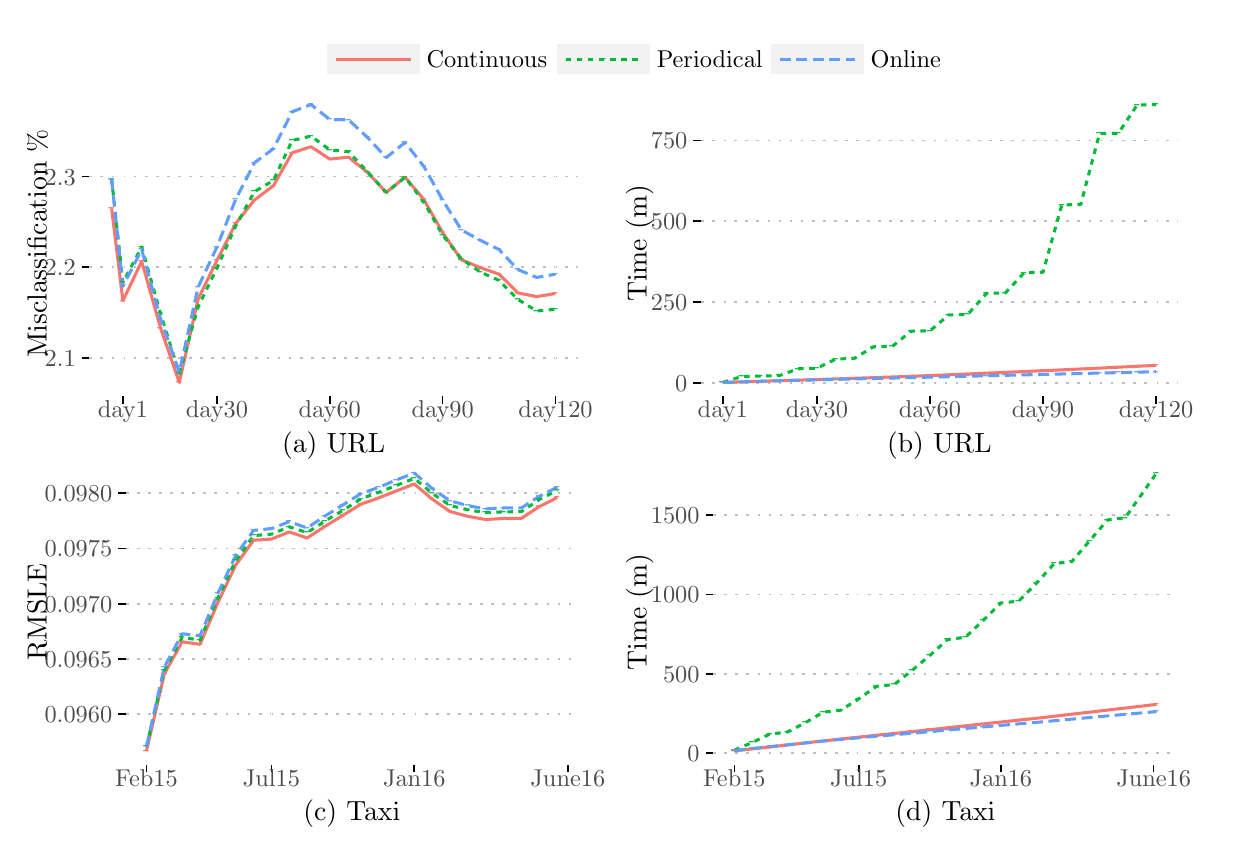
\begin{tikzpicture}[x=1pt,y=1pt]
\definecolor{fillColor}{RGB}{255,255,255}
\path[use as bounding box,fill=fillColor,fill opacity=0.00] (0,0) rectangle (433.62,289.08);
\begin{scope}
\path[clip] (  0.00,  0.00) rectangle (433.62,289.08);
\definecolor{fillColor}{RGB}{255,255,255}

\path[fill=fillColor] ( 97.81,266.32) rectangle (335.81,289.08);
\end{scope}
\begin{scope}
\path[clip] (  0.00,  0.00) rectangle (433.62,289.08);
\definecolor{drawColor}{RGB}{255,255,255}
\definecolor{fillColor}{gray}{0.95}

\path[draw=drawColor,line width= 0.6pt,line join=round,line cap=round,fill=fillColor] (107.84,272.01) rectangle (141.98,283.39);
\end{scope}
\begin{scope}
\path[clip] (  0.00,  0.00) rectangle (433.62,289.08);
\definecolor{drawColor}{RGB}{248,118,109}

\path[draw=drawColor,line width= 1.1pt,line join=round] (111.25,277.70) -- (138.57,277.70);
\end{scope}
\begin{scope}
\path[clip] (  0.00,  0.00) rectangle (433.62,289.08);
\definecolor{drawColor}{RGB}{248,118,109}

\node[text=drawColor,anchor=base,inner sep=0pt, outer sep=0pt, scale=  0.72] at (124.91,276.15) {-};
\end{scope}
\begin{scope}
\path[clip] (  0.00,  0.00) rectangle (433.62,289.08);
\definecolor{drawColor}{RGB}{255,255,255}
\definecolor{fillColor}{gray}{0.95}

\path[draw=drawColor,line width= 0.6pt,line join=round,line cap=round,fill=fillColor] (191.01,272.01) rectangle (225.15,283.39);
\end{scope}
\begin{scope}
\path[clip] (  0.00,  0.00) rectangle (433.62,289.08);
\definecolor{drawColor}{RGB}{0,186,56}

\path[draw=drawColor,line width= 1.1pt,dash pattern=on 2pt off 2pt ,line join=round] (194.42,277.70) -- (221.74,277.70);
\end{scope}
\begin{scope}
\path[clip] (  0.00,  0.00) rectangle (433.62,289.08);
\definecolor{drawColor}{RGB}{0,186,56}

\node[text=drawColor,anchor=base,inner sep=0pt, outer sep=0pt, scale=  0.72] at (208.08,276.15) {-};
\end{scope}
\begin{scope}
\path[clip] (  0.00,  0.00) rectangle (433.62,289.08);
\definecolor{drawColor}{RGB}{255,255,255}
\definecolor{fillColor}{gray}{0.95}

\path[draw=drawColor,line width= 0.6pt,line join=round,line cap=round,fill=fillColor] (268.27,272.01) rectangle (302.42,283.39);
\end{scope}
\begin{scope}
\path[clip] (  0.00,  0.00) rectangle (433.62,289.08);
\definecolor{drawColor}{RGB}{97,156,255}

\path[draw=drawColor,line width= 1.1pt,dash pattern=on 4pt off 2pt ,line join=round] (271.69,277.70) -- (299.00,277.70);
\end{scope}
\begin{scope}
\path[clip] (  0.00,  0.00) rectangle (433.62,289.08);
\definecolor{drawColor}{RGB}{97,156,255}

\node[text=drawColor,anchor=base,inner sep=0pt, outer sep=0pt, scale=  0.72] at (285.34,276.15) {-};
\end{scope}
\begin{scope}
\path[clip] (  0.00,  0.00) rectangle (433.62,289.08);
\definecolor{drawColor}{RGB}{0,0,0}

\node[text=drawColor,anchor=base west,inner sep=0pt, outer sep=0pt, scale=  0.88] at (144.15,274.67) {Continuous};
\end{scope}
\begin{scope}
\path[clip] (  0.00,  0.00) rectangle (433.62,289.08);
\definecolor{drawColor}{RGB}{0,0,0}

\node[text=drawColor,anchor=base west,inner sep=0pt, outer sep=0pt, scale=  0.88] at (227.32,274.67) {Periodical};
\end{scope}
\begin{scope}
\path[clip] (  0.00,  0.00) rectangle (433.62,289.08);
\definecolor{drawColor}{RGB}{0,0,0}

\node[text=drawColor,anchor=base west,inner sep=0pt, outer sep=0pt, scale=  0.88] at (304.58,274.67) {Online};
\end{scope}
\begin{scope}
\path[clip] (  0.00,133.16) rectangle (216.81,266.32);
\definecolor{drawColor}{RGB}{255,255,255}
\definecolor{fillColor}{RGB}{255,255,255}

\path[draw=drawColor,line width= 0.6pt,line join=round,line cap=round,fill=fillColor] (  0.00,133.16) rectangle (216.81,266.32);
\end{scope}
\begin{scope}
\path[clip] ( 22.31,155.85) rectangle (198.74,266.32);
\definecolor{fillColor}{RGB}{255,255,255}

\path[fill=fillColor] ( 22.31,155.85) rectangle (198.74,266.32);
\definecolor{drawColor}{RGB}{255,255,255}

\path[draw=drawColor,line width= 0.3pt,line join=round] ( 22.31,186.15) --
	(198.74,186.15);

\path[draw=drawColor,line width= 0.3pt,line join=round] ( 22.31,218.88) --
	(198.74,218.88);

\path[draw=drawColor,line width= 0.3pt,line join=round] ( 22.31,251.60) --
	(198.74,251.60);

\path[draw=drawColor,line width= 0.3pt,line join=round] ( 51.40,155.85) --
	( 51.40,266.32);

\path[draw=drawColor,line width= 0.3pt,line join=round] ( 88.78,155.85) --
	( 88.78,266.32);

\path[draw=drawColor,line width= 0.3pt,line join=round] (129.56,155.85) --
	(129.56,266.32);

\path[draw=drawColor,line width= 0.3pt,line join=round] (170.33,155.85) --
	(170.33,266.32);
\definecolor{drawColor}{RGB}{190,190,190}

\path[draw=drawColor,line width= 0.6pt,dash pattern=on 1pt off 3pt ,line join=round] ( 22.31,169.79) --
	(198.74,169.79);

\path[draw=drawColor,line width= 0.6pt,dash pattern=on 1pt off 3pt ,line join=round] ( 22.31,202.51) --
	(198.74,202.51);

\path[draw=drawColor,line width= 0.6pt,dash pattern=on 1pt off 3pt ,line join=round] ( 22.31,235.24) --
	(198.74,235.24);
\definecolor{drawColor}{RGB}{255,255,255}

\path[draw=drawColor,line width= 0.6pt,line join=round] ( 34.41,155.85) --
	( 34.41,266.32);

\path[draw=drawColor,line width= 0.6pt,line join=round] ( 68.39,155.85) --
	( 68.39,266.32);

\path[draw=drawColor,line width= 0.6pt,line join=round] (109.17,155.85) --
	(109.17,266.32);

\path[draw=drawColor,line width= 0.6pt,line join=round] (149.94,155.85) --
	(149.94,266.32);

\path[draw=drawColor,line width= 0.6pt,line join=round] (190.72,155.85) --
	(190.72,266.32);
\definecolor{drawColor}{RGB}{248,118,109}

\path[draw=drawColor,line width= 1.1pt,line join=round] ( 30.33,223.79) --
	( 34.41,190.41) --
	( 41.20,204.64) --
	( 48.00,180.59) --
	( 54.79,160.87) --
	( 61.59,191.06) --
	( 68.39,204.97) --
	( 75.18,218.32) --
	( 81.98,226.85) --
	( 88.78,231.93) --
	( 95.57,243.85) --
	(102.37,246.06) --
	(109.17,241.59) --
	(115.96,242.27) --
	(122.76,236.85) --
	(129.56,229.54) --
	(136.35,235.07) --
	(143.15,226.98) --
	(149.94,215.02) --
	(156.74,205.20) --
	(163.54,202.38) --
	(170.33,200.00) --
	(177.13,193.24) --
	(183.93,191.90) --
	(190.72,193.00);
\definecolor{drawColor}{RGB}{0,186,56}

\path[draw=drawColor,line width= 1.1pt,dash pattern=on 2pt off 2pt ,line join=round] ( 30.33,234.42) --
	( 34.41,196.95) --
	( 41.20,209.88) --
	( 48.00,185.82) --
	( 54.79,164.14) --
	( 61.59,188.18) --
	( 68.39,202.19) --
	( 75.18,217.48) --
	( 81.98,229.88) --
	( 88.78,233.81) --
	( 95.57,248.30) --
	(102.37,249.91) --
	(109.17,244.92) --
	(115.96,244.26) --
	(122.76,237.00) --
	(129.56,229.51) --
	(136.35,234.99) --
	(143.15,226.07) --
	(149.94,214.14) --
	(156.74,205.49) --
	(163.54,200.81) --
	(170.33,197.75) --
	(177.13,190.88) --
	(183.93,186.71) --
	(190.72,187.32);
\definecolor{drawColor}{RGB}{97,156,255}

\path[draw=drawColor,line width= 1.1pt,dash pattern=on 4pt off 2pt ,line join=round] ( 30.33,234.42) --
	( 34.41,195.64) --
	( 41.20,208.90) --
	( 48.00,183.86) --
	( 54.79,164.63) --
	( 61.59,195.32) --
	( 68.39,209.82) --
	( 75.18,227.06) --
	( 81.98,240.27) --
	( 88.78,245.32) --
	( 95.57,258.68) --
	(102.37,261.30) --
	(109.17,255.90) --
	(115.96,255.77) --
	(122.76,249.47) --
	(129.56,242.12) --
	(136.35,247.58) --
	(143.15,238.96) --
	(149.94,226.77) --
	(156.74,215.99) --
	(163.54,212.25) --
	(170.33,208.90) --
	(177.13,201.68) --
	(183.93,198.83) --
	(190.72,200.00);
\definecolor{drawColor}{RGB}{248,118,109}

\node[text=drawColor,anchor=base,inner sep=0pt, outer sep=0pt, scale=  0.72] at ( 30.33,222.24) {-};

\node[text=drawColor,anchor=base,inner sep=0pt, outer sep=0pt, scale=  0.72] at ( 34.41,188.86) {-};

\node[text=drawColor,anchor=base,inner sep=0pt, outer sep=0pt, scale=  0.72] at ( 41.20,203.09) {-};

\node[text=drawColor,anchor=base,inner sep=0pt, outer sep=0pt, scale=  0.72] at ( 48.00,179.04) {-};

\node[text=drawColor,anchor=base,inner sep=0pt, outer sep=0pt, scale=  0.72] at ( 54.79,159.32) {-};

\node[text=drawColor,anchor=base,inner sep=0pt, outer sep=0pt, scale=  0.72] at ( 61.59,189.51) {-};

\node[text=drawColor,anchor=base,inner sep=0pt, outer sep=0pt, scale=  0.72] at ( 68.39,203.42) {-};

\node[text=drawColor,anchor=base,inner sep=0pt, outer sep=0pt, scale=  0.72] at ( 75.18,216.77) {-};

\node[text=drawColor,anchor=base,inner sep=0pt, outer sep=0pt, scale=  0.72] at ( 81.98,225.30) {-};

\node[text=drawColor,anchor=base,inner sep=0pt, outer sep=0pt, scale=  0.72] at ( 88.78,230.38) {-};

\node[text=drawColor,anchor=base,inner sep=0pt, outer sep=0pt, scale=  0.72] at ( 95.57,242.30) {-};

\node[text=drawColor,anchor=base,inner sep=0pt, outer sep=0pt, scale=  0.72] at (102.37,244.51) {-};

\node[text=drawColor,anchor=base,inner sep=0pt, outer sep=0pt, scale=  0.72] at (109.17,240.04) {-};

\node[text=drawColor,anchor=base,inner sep=0pt, outer sep=0pt, scale=  0.72] at (115.96,240.72) {-};

\node[text=drawColor,anchor=base,inner sep=0pt, outer sep=0pt, scale=  0.72] at (122.76,235.30) {-};

\node[text=drawColor,anchor=base,inner sep=0pt, outer sep=0pt, scale=  0.72] at (129.56,227.99) {-};

\node[text=drawColor,anchor=base,inner sep=0pt, outer sep=0pt, scale=  0.72] at (136.35,233.52) {-};

\node[text=drawColor,anchor=base,inner sep=0pt, outer sep=0pt, scale=  0.72] at (143.15,225.43) {-};

\node[text=drawColor,anchor=base,inner sep=0pt, outer sep=0pt, scale=  0.72] at (149.94,213.47) {-};

\node[text=drawColor,anchor=base,inner sep=0pt, outer sep=0pt, scale=  0.72] at (156.74,203.65) {-};

\node[text=drawColor,anchor=base,inner sep=0pt, outer sep=0pt, scale=  0.72] at (163.54,200.83) {-};

\node[text=drawColor,anchor=base,inner sep=0pt, outer sep=0pt, scale=  0.72] at (170.33,198.45) {-};

\node[text=drawColor,anchor=base,inner sep=0pt, outer sep=0pt, scale=  0.72] at (177.13,191.69) {-};

\node[text=drawColor,anchor=base,inner sep=0pt, outer sep=0pt, scale=  0.72] at (183.93,190.35) {-};

\node[text=drawColor,anchor=base,inner sep=0pt, outer sep=0pt, scale=  0.72] at (190.72,191.45) {-};
\definecolor{drawColor}{RGB}{0,186,56}

\node[text=drawColor,anchor=base,inner sep=0pt, outer sep=0pt, scale=  0.72] at ( 30.33,232.87) {-};

\node[text=drawColor,anchor=base,inner sep=0pt, outer sep=0pt, scale=  0.72] at ( 34.41,195.40) {-};

\node[text=drawColor,anchor=base,inner sep=0pt, outer sep=0pt, scale=  0.72] at ( 41.20,208.33) {-};

\node[text=drawColor,anchor=base,inner sep=0pt, outer sep=0pt, scale=  0.72] at ( 48.00,184.27) {-};

\node[text=drawColor,anchor=base,inner sep=0pt, outer sep=0pt, scale=  0.72] at ( 54.79,162.59) {-};

\node[text=drawColor,anchor=base,inner sep=0pt, outer sep=0pt, scale=  0.72] at ( 61.59,186.63) {-};

\node[text=drawColor,anchor=base,inner sep=0pt, outer sep=0pt, scale=  0.72] at ( 68.39,200.64) {-};

\node[text=drawColor,anchor=base,inner sep=0pt, outer sep=0pt, scale=  0.72] at ( 75.18,215.92) {-};

\node[text=drawColor,anchor=base,inner sep=0pt, outer sep=0pt, scale=  0.72] at ( 81.98,228.33) {-};

\node[text=drawColor,anchor=base,inner sep=0pt, outer sep=0pt, scale=  0.72] at ( 88.78,232.26) {-};

\node[text=drawColor,anchor=base,inner sep=0pt, outer sep=0pt, scale=  0.72] at ( 95.57,246.74) {-};

\node[text=drawColor,anchor=base,inner sep=0pt, outer sep=0pt, scale=  0.72] at (102.37,248.35) {-};

\node[text=drawColor,anchor=base,inner sep=0pt, outer sep=0pt, scale=  0.72] at (109.17,243.37) {-};

\node[text=drawColor,anchor=base,inner sep=0pt, outer sep=0pt, scale=  0.72] at (115.96,242.71) {-};

\node[text=drawColor,anchor=base,inner sep=0pt, outer sep=0pt, scale=  0.72] at (122.76,235.44) {-};

\node[text=drawColor,anchor=base,inner sep=0pt, outer sep=0pt, scale=  0.72] at (129.56,227.96) {-};

\node[text=drawColor,anchor=base,inner sep=0pt, outer sep=0pt, scale=  0.72] at (136.35,233.44) {-};

\node[text=drawColor,anchor=base,inner sep=0pt, outer sep=0pt, scale=  0.72] at (143.15,224.52) {-};

\node[text=drawColor,anchor=base,inner sep=0pt, outer sep=0pt, scale=  0.72] at (149.94,212.59) {-};

\node[text=drawColor,anchor=base,inner sep=0pt, outer sep=0pt, scale=  0.72] at (156.74,203.94) {-};

\node[text=drawColor,anchor=base,inner sep=0pt, outer sep=0pt, scale=  0.72] at (163.54,199.26) {-};

\node[text=drawColor,anchor=base,inner sep=0pt, outer sep=0pt, scale=  0.72] at (170.33,196.20) {-};

\node[text=drawColor,anchor=base,inner sep=0pt, outer sep=0pt, scale=  0.72] at (177.13,189.33) {-};

\node[text=drawColor,anchor=base,inner sep=0pt, outer sep=0pt, scale=  0.72] at (183.93,185.16) {-};

\node[text=drawColor,anchor=base,inner sep=0pt, outer sep=0pt, scale=  0.72] at (190.72,185.77) {-};
\definecolor{drawColor}{RGB}{97,156,255}

\node[text=drawColor,anchor=base,inner sep=0pt, outer sep=0pt, scale=  0.72] at ( 30.33,232.87) {-};

\node[text=drawColor,anchor=base,inner sep=0pt, outer sep=0pt, scale=  0.72] at ( 34.41,194.09) {-};

\node[text=drawColor,anchor=base,inner sep=0pt, outer sep=0pt, scale=  0.72] at ( 41.20,207.35) {-};

\node[text=drawColor,anchor=base,inner sep=0pt, outer sep=0pt, scale=  0.72] at ( 48.00,182.31) {-};

\node[text=drawColor,anchor=base,inner sep=0pt, outer sep=0pt, scale=  0.72] at ( 54.79,163.08) {-};

\node[text=drawColor,anchor=base,inner sep=0pt, outer sep=0pt, scale=  0.72] at ( 61.59,193.76) {-};

\node[text=drawColor,anchor=base,inner sep=0pt, outer sep=0pt, scale=  0.72] at ( 68.39,208.27) {-};

\node[text=drawColor,anchor=base,inner sep=0pt, outer sep=0pt, scale=  0.72] at ( 75.18,225.51) {-};

\node[text=drawColor,anchor=base,inner sep=0pt, outer sep=0pt, scale=  0.72] at ( 81.98,238.72) {-};

\node[text=drawColor,anchor=base,inner sep=0pt, outer sep=0pt, scale=  0.72] at ( 88.78,243.77) {-};

\node[text=drawColor,anchor=base,inner sep=0pt, outer sep=0pt, scale=  0.72] at ( 95.57,257.13) {-};

\node[text=drawColor,anchor=base,inner sep=0pt, outer sep=0pt, scale=  0.72] at (102.37,259.75) {-};

\node[text=drawColor,anchor=base,inner sep=0pt, outer sep=0pt, scale=  0.72] at (109.17,254.35) {-};

\node[text=drawColor,anchor=base,inner sep=0pt, outer sep=0pt, scale=  0.72] at (115.96,254.22) {-};

\node[text=drawColor,anchor=base,inner sep=0pt, outer sep=0pt, scale=  0.72] at (122.76,247.92) {-};

\node[text=drawColor,anchor=base,inner sep=0pt, outer sep=0pt, scale=  0.72] at (129.56,240.57) {-};

\node[text=drawColor,anchor=base,inner sep=0pt, outer sep=0pt, scale=  0.72] at (136.35,246.03) {-};

\node[text=drawColor,anchor=base,inner sep=0pt, outer sep=0pt, scale=  0.72] at (143.15,237.41) {-};

\node[text=drawColor,anchor=base,inner sep=0pt, outer sep=0pt, scale=  0.72] at (149.94,225.22) {-};

\node[text=drawColor,anchor=base,inner sep=0pt, outer sep=0pt, scale=  0.72] at (156.74,214.44) {-};

\node[text=drawColor,anchor=base,inner sep=0pt, outer sep=0pt, scale=  0.72] at (163.54,210.70) {-};

\node[text=drawColor,anchor=base,inner sep=0pt, outer sep=0pt, scale=  0.72] at (170.33,207.35) {-};

\node[text=drawColor,anchor=base,inner sep=0pt, outer sep=0pt, scale=  0.72] at (177.13,200.13) {-};

\node[text=drawColor,anchor=base,inner sep=0pt, outer sep=0pt, scale=  0.72] at (183.93,197.28) {-};

\node[text=drawColor,anchor=base,inner sep=0pt, outer sep=0pt, scale=  0.72] at (190.72,198.45) {-};
\end{scope}
\begin{scope}
\path[clip] (  0.00,  0.00) rectangle (433.62,289.08);
\definecolor{drawColor}{gray}{0.30}

\node[text=drawColor,anchor=base east,inner sep=0pt, outer sep=0pt, scale=  0.88] at ( 17.36,166.76) {2.1};

\node[text=drawColor,anchor=base east,inner sep=0pt, outer sep=0pt, scale=  0.88] at ( 17.36,199.48) {2.2};

\node[text=drawColor,anchor=base east,inner sep=0pt, outer sep=0pt, scale=  0.88] at ( 17.36,232.21) {2.3};
\end{scope}
\begin{scope}
\path[clip] (  0.00,  0.00) rectangle (433.62,289.08);
\definecolor{drawColor}{RGB}{0,0,0}

\path[draw=drawColor,line width= 0.6pt,line join=round] ( 19.56,169.79) --
	( 22.31,169.79);

\path[draw=drawColor,line width= 0.6pt,line join=round] ( 19.56,202.51) --
	( 22.31,202.51);

\path[draw=drawColor,line width= 0.6pt,line join=round] ( 19.56,235.24) --
	( 22.31,235.24);
\end{scope}
\begin{scope}
\path[clip] (  0.00,  0.00) rectangle (433.62,289.08);
\definecolor{drawColor}{RGB}{0,0,0}

\path[draw=drawColor,line width= 0.6pt,line join=round] ( 34.41,153.10) --
	( 34.41,155.85);

\path[draw=drawColor,line width= 0.6pt,line join=round] ( 68.39,153.10) --
	( 68.39,155.85);

\path[draw=drawColor,line width= 0.6pt,line join=round] (109.17,153.10) --
	(109.17,155.85);

\path[draw=drawColor,line width= 0.6pt,line join=round] (149.94,153.10) --
	(149.94,155.85);

\path[draw=drawColor,line width= 0.6pt,line join=round] (190.72,153.10) --
	(190.72,155.85);
\end{scope}
\begin{scope}
\path[clip] (  0.00,  0.00) rectangle (433.62,289.08);
\definecolor{drawColor}{gray}{0.30}

\node[text=drawColor,anchor=base,inner sep=0pt, outer sep=0pt, scale=  0.88] at ( 34.41,148.04) {day1};

\node[text=drawColor,anchor=base,inner sep=0pt, outer sep=0pt, scale=  0.88] at ( 68.39,148.04) {day30};

\node[text=drawColor,anchor=base,inner sep=0pt, outer sep=0pt, scale=  0.88] at (109.17,148.04) {day60};

\node[text=drawColor,anchor=base,inner sep=0pt, outer sep=0pt, scale=  0.88] at (149.94,148.04) {day90};

\node[text=drawColor,anchor=base,inner sep=0pt, outer sep=0pt, scale=  0.88] at (190.72,148.04) {day120};
\end{scope}
\begin{scope}
\path[clip] (  0.00,  0.00) rectangle (433.62,289.08);
\definecolor{drawColor}{RGB}{0,0,0}

\node[text=drawColor,anchor=base,inner sep=0pt, outer sep=0pt, scale=  1.00] at (110.53,135.65) {(a) URL};
\end{scope}
\begin{scope}
\path[clip] (  0.00,  0.00) rectangle (433.62,289.08);
\definecolor{drawColor}{RGB}{0,0,0}

\node[text=drawColor,rotate= 90.00,anchor=base,inner sep=0pt, outer sep=0pt, scale=  1.00] at (  6.89,211.08) {Misclassification \%};
\end{scope}
\begin{scope}
\path[clip] (216.81,133.16) rectangle (433.62,266.32);
\definecolor{drawColor}{RGB}{255,255,255}
\definecolor{fillColor}{RGB}{255,255,255}

\path[draw=drawColor,line width= 0.6pt,line join=round,line cap=round,fill=fillColor] (216.81,133.16) rectangle (433.62,266.32);
\end{scope}
\begin{scope}
\path[clip] (243.34,155.85) rectangle (415.55,266.32);
\definecolor{fillColor}{RGB}{255,255,255}

\path[fill=fillColor] (243.34,155.85) rectangle (415.55,266.32);
\definecolor{drawColor}{RGB}{255,255,255}

\path[draw=drawColor,line width= 0.3pt,line join=round] (243.34,175.29) --
	(415.55,175.29);

\path[draw=drawColor,line width= 0.3pt,line join=round] (243.34,204.50) --
	(415.55,204.50);

\path[draw=drawColor,line width= 0.3pt,line join=round] (243.34,233.72) --
	(415.55,233.72);

\path[draw=drawColor,line width= 0.3pt,line join=round] (243.34,262.93) --
	(415.55,262.93);

\path[draw=drawColor,line width= 0.3pt,line join=round] (268.18,155.85) --
	(268.18,266.32);

\path[draw=drawColor,line width= 0.3pt,line join=round] (305.62,155.85) --
	(305.62,266.32);

\path[draw=drawColor,line width= 0.3pt,line join=round] (346.46,155.85) --
	(346.46,266.32);

\path[draw=drawColor,line width= 0.3pt,line join=round] (387.30,155.85) --
	(387.30,266.32);
\definecolor{drawColor}{RGB}{190,190,190}

\path[draw=drawColor,line width= 0.6pt,dash pattern=on 1pt off 3pt ,line join=round] (243.34,160.69) --
	(415.55,160.69);

\path[draw=drawColor,line width= 0.6pt,dash pattern=on 1pt off 3pt ,line join=round] (243.34,189.90) --
	(415.55,189.90);

\path[draw=drawColor,line width= 0.6pt,dash pattern=on 1pt off 3pt ,line join=round] (243.34,219.11) --
	(415.55,219.11);

\path[draw=drawColor,line width= 0.6pt,dash pattern=on 1pt off 3pt ,line join=round] (243.34,248.32) --
	(415.55,248.32);
\definecolor{drawColor}{RGB}{255,255,255}

\path[draw=drawColor,line width= 0.6pt,line join=round] (251.17,155.85) --
	(251.17,266.32);

\path[draw=drawColor,line width= 0.6pt,line join=round] (285.20,155.85) --
	(285.20,266.32);

\path[draw=drawColor,line width= 0.6pt,line join=round] (326.04,155.85) --
	(326.04,266.32);

\path[draw=drawColor,line width= 0.6pt,line join=round] (366.88,155.85) --
	(366.88,266.32);

\path[draw=drawColor,line width= 0.6pt,line join=round] (407.72,155.85) --
	(407.72,266.32);
\definecolor{drawColor}{RGB}{248,118,109}

\path[draw=drawColor,line width= 1.1pt,line join=round] (251.17,160.89) --
	(257.97,161.09) --
	(264.78,161.30) --
	(271.59,161.50) --
	(278.39,161.71) --
	(285.20,161.92) --
	(292.01,162.16) --
	(298.81,162.39) --
	(305.62,162.61) --
	(312.43,162.86) --
	(319.23,163.10) --
	(326.04,163.37) --
	(332.85,163.65) --
	(339.66,163.95) --
	(346.46,164.24) --
	(353.27,164.53) --
	(360.08,164.82) --
	(366.88,165.13) --
	(373.69,165.43) --
	(380.50,165.75) --
	(387.30,166.06) --
	(394.11,166.39) --
	(400.92,166.72) --
	(407.72,167.07);
\definecolor{drawColor}{RGB}{0,186,56}

\path[draw=drawColor,line width= 1.1pt,dash pattern=on 2pt off 2pt ,line join=round] (251.17,160.90) --
	(257.97,163.01) --
	(264.78,163.18) --
	(271.59,163.35) --
	(278.39,165.82) --
	(285.20,166.03) --
	(292.01,169.31) --
	(298.81,169.62) --
	(305.62,173.77) --
	(312.43,173.93) --
	(319.23,179.39) --
	(326.04,179.54) --
	(332.85,185.30) --
	(339.66,185.45) --
	(346.46,193.05) --
	(353.27,193.23) --
	(360.08,200.53) --
	(366.88,200.71) --
	(373.69,225.03) --
	(380.50,225.17) --
	(387.30,250.78) --
	(394.11,250.93) --
	(400.92,261.15) --
	(407.72,261.30);
\definecolor{drawColor}{RGB}{97,156,255}

\path[draw=drawColor,line width= 1.1pt,dash pattern=on 4pt off 2pt ,line join=round] (251.17,160.87) --
	(257.97,161.04) --
	(264.78,161.32) --
	(271.59,161.49) --
	(278.39,161.66) --
	(285.20,161.82) --
	(292.01,161.99) --
	(298.81,162.16) --
	(305.62,162.30) --
	(312.43,162.47) --
	(319.23,162.63) --
	(326.04,162.80) --
	(332.85,162.96) --
	(339.66,163.13) --
	(346.46,163.29) --
	(353.27,163.45) --
	(360.08,163.62) --
	(366.88,163.78) --
	(373.69,163.94) --
	(380.50,164.11) --
	(387.30,164.27) --
	(394.11,164.43) --
	(400.92,164.60) --
	(407.72,164.76);
\definecolor{drawColor}{RGB}{248,118,109}

\node[text=drawColor,anchor=base,inner sep=0pt, outer sep=0pt, scale=  0.72] at (251.17,159.34) {-};

\node[text=drawColor,anchor=base,inner sep=0pt, outer sep=0pt, scale=  0.72] at (257.97,159.54) {-};

\node[text=drawColor,anchor=base,inner sep=0pt, outer sep=0pt, scale=  0.72] at (264.78,159.75) {-};

\node[text=drawColor,anchor=base,inner sep=0pt, outer sep=0pt, scale=  0.72] at (271.59,159.95) {-};

\node[text=drawColor,anchor=base,inner sep=0pt, outer sep=0pt, scale=  0.72] at (278.39,160.16) {-};

\node[text=drawColor,anchor=base,inner sep=0pt, outer sep=0pt, scale=  0.72] at (285.20,160.37) {-};

\node[text=drawColor,anchor=base,inner sep=0pt, outer sep=0pt, scale=  0.72] at (292.01,160.61) {-};

\node[text=drawColor,anchor=base,inner sep=0pt, outer sep=0pt, scale=  0.72] at (298.81,160.84) {-};

\node[text=drawColor,anchor=base,inner sep=0pt, outer sep=0pt, scale=  0.72] at (305.62,161.06) {-};

\node[text=drawColor,anchor=base,inner sep=0pt, outer sep=0pt, scale=  0.72] at (312.43,161.31) {-};

\node[text=drawColor,anchor=base,inner sep=0pt, outer sep=0pt, scale=  0.72] at (319.23,161.55) {-};

\node[text=drawColor,anchor=base,inner sep=0pt, outer sep=0pt, scale=  0.72] at (326.04,161.82) {-};

\node[text=drawColor,anchor=base,inner sep=0pt, outer sep=0pt, scale=  0.72] at (332.85,162.10) {-};

\node[text=drawColor,anchor=base,inner sep=0pt, outer sep=0pt, scale=  0.72] at (339.66,162.40) {-};

\node[text=drawColor,anchor=base,inner sep=0pt, outer sep=0pt, scale=  0.72] at (346.46,162.69) {-};

\node[text=drawColor,anchor=base,inner sep=0pt, outer sep=0pt, scale=  0.72] at (353.27,162.98) {-};

\node[text=drawColor,anchor=base,inner sep=0pt, outer sep=0pt, scale=  0.72] at (360.08,163.27) {-};

\node[text=drawColor,anchor=base,inner sep=0pt, outer sep=0pt, scale=  0.72] at (366.88,163.58) {-};

\node[text=drawColor,anchor=base,inner sep=0pt, outer sep=0pt, scale=  0.72] at (373.69,163.88) {-};

\node[text=drawColor,anchor=base,inner sep=0pt, outer sep=0pt, scale=  0.72] at (380.50,164.19) {-};

\node[text=drawColor,anchor=base,inner sep=0pt, outer sep=0pt, scale=  0.72] at (387.30,164.51) {-};

\node[text=drawColor,anchor=base,inner sep=0pt, outer sep=0pt, scale=  0.72] at (394.11,164.84) {-};

\node[text=drawColor,anchor=base,inner sep=0pt, outer sep=0pt, scale=  0.72] at (400.92,165.17) {-};

\node[text=drawColor,anchor=base,inner sep=0pt, outer sep=0pt, scale=  0.72] at (407.72,165.52) {-};
\definecolor{drawColor}{RGB}{0,186,56}

\node[text=drawColor,anchor=base,inner sep=0pt, outer sep=0pt, scale=  0.72] at (251.17,159.35) {-};

\node[text=drawColor,anchor=base,inner sep=0pt, outer sep=0pt, scale=  0.72] at (257.97,161.46) {-};

\node[text=drawColor,anchor=base,inner sep=0pt, outer sep=0pt, scale=  0.72] at (264.78,161.63) {-};

\node[text=drawColor,anchor=base,inner sep=0pt, outer sep=0pt, scale=  0.72] at (271.59,161.80) {-};

\node[text=drawColor,anchor=base,inner sep=0pt, outer sep=0pt, scale=  0.72] at (278.39,164.27) {-};

\node[text=drawColor,anchor=base,inner sep=0pt, outer sep=0pt, scale=  0.72] at (285.20,164.47) {-};

\node[text=drawColor,anchor=base,inner sep=0pt, outer sep=0pt, scale=  0.72] at (292.01,167.76) {-};

\node[text=drawColor,anchor=base,inner sep=0pt, outer sep=0pt, scale=  0.72] at (298.81,168.07) {-};

\node[text=drawColor,anchor=base,inner sep=0pt, outer sep=0pt, scale=  0.72] at (305.62,172.22) {-};

\node[text=drawColor,anchor=base,inner sep=0pt, outer sep=0pt, scale=  0.72] at (312.43,172.38) {-};

\node[text=drawColor,anchor=base,inner sep=0pt, outer sep=0pt, scale=  0.72] at (319.23,177.83) {-};

\node[text=drawColor,anchor=base,inner sep=0pt, outer sep=0pt, scale=  0.72] at (326.04,177.99) {-};

\node[text=drawColor,anchor=base,inner sep=0pt, outer sep=0pt, scale=  0.72] at (332.85,183.75) {-};

\node[text=drawColor,anchor=base,inner sep=0pt, outer sep=0pt, scale=  0.72] at (339.66,183.90) {-};

\node[text=drawColor,anchor=base,inner sep=0pt, outer sep=0pt, scale=  0.72] at (346.46,191.50) {-};

\node[text=drawColor,anchor=base,inner sep=0pt, outer sep=0pt, scale=  0.72] at (353.27,191.68) {-};

\node[text=drawColor,anchor=base,inner sep=0pt, outer sep=0pt, scale=  0.72] at (360.08,198.98) {-};

\node[text=drawColor,anchor=base,inner sep=0pt, outer sep=0pt, scale=  0.72] at (366.88,199.16) {-};

\node[text=drawColor,anchor=base,inner sep=0pt, outer sep=0pt, scale=  0.72] at (373.69,223.48) {-};

\node[text=drawColor,anchor=base,inner sep=0pt, outer sep=0pt, scale=  0.72] at (380.50,223.62) {-};

\node[text=drawColor,anchor=base,inner sep=0pt, outer sep=0pt, scale=  0.72] at (387.30,249.23) {-};

\node[text=drawColor,anchor=base,inner sep=0pt, outer sep=0pt, scale=  0.72] at (394.11,249.38) {-};

\node[text=drawColor,anchor=base,inner sep=0pt, outer sep=0pt, scale=  0.72] at (400.92,259.60) {-};

\node[text=drawColor,anchor=base,inner sep=0pt, outer sep=0pt, scale=  0.72] at (407.72,259.75) {-};
\definecolor{drawColor}{RGB}{97,156,255}

\node[text=drawColor,anchor=base,inner sep=0pt, outer sep=0pt, scale=  0.72] at (251.17,159.32) {-};

\node[text=drawColor,anchor=base,inner sep=0pt, outer sep=0pt, scale=  0.72] at (257.97,159.49) {-};

\node[text=drawColor,anchor=base,inner sep=0pt, outer sep=0pt, scale=  0.72] at (264.78,159.77) {-};

\node[text=drawColor,anchor=base,inner sep=0pt, outer sep=0pt, scale=  0.72] at (271.59,159.94) {-};

\node[text=drawColor,anchor=base,inner sep=0pt, outer sep=0pt, scale=  0.72] at (278.39,160.11) {-};

\node[text=drawColor,anchor=base,inner sep=0pt, outer sep=0pt, scale=  0.72] at (285.20,160.27) {-};

\node[text=drawColor,anchor=base,inner sep=0pt, outer sep=0pt, scale=  0.72] at (292.01,160.44) {-};

\node[text=drawColor,anchor=base,inner sep=0pt, outer sep=0pt, scale=  0.72] at (298.81,160.61) {-};

\node[text=drawColor,anchor=base,inner sep=0pt, outer sep=0pt, scale=  0.72] at (305.62,160.75) {-};

\node[text=drawColor,anchor=base,inner sep=0pt, outer sep=0pt, scale=  0.72] at (312.43,160.92) {-};

\node[text=drawColor,anchor=base,inner sep=0pt, outer sep=0pt, scale=  0.72] at (319.23,161.08) {-};

\node[text=drawColor,anchor=base,inner sep=0pt, outer sep=0pt, scale=  0.72] at (326.04,161.25) {-};

\node[text=drawColor,anchor=base,inner sep=0pt, outer sep=0pt, scale=  0.72] at (332.85,161.41) {-};

\node[text=drawColor,anchor=base,inner sep=0pt, outer sep=0pt, scale=  0.72] at (339.66,161.58) {-};

\node[text=drawColor,anchor=base,inner sep=0pt, outer sep=0pt, scale=  0.72] at (346.46,161.74) {-};

\node[text=drawColor,anchor=base,inner sep=0pt, outer sep=0pt, scale=  0.72] at (353.27,161.90) {-};

\node[text=drawColor,anchor=base,inner sep=0pt, outer sep=0pt, scale=  0.72] at (360.08,162.07) {-};

\node[text=drawColor,anchor=base,inner sep=0pt, outer sep=0pt, scale=  0.72] at (366.88,162.23) {-};

\node[text=drawColor,anchor=base,inner sep=0pt, outer sep=0pt, scale=  0.72] at (373.69,162.39) {-};

\node[text=drawColor,anchor=base,inner sep=0pt, outer sep=0pt, scale=  0.72] at (380.50,162.56) {-};

\node[text=drawColor,anchor=base,inner sep=0pt, outer sep=0pt, scale=  0.72] at (387.30,162.72) {-};

\node[text=drawColor,anchor=base,inner sep=0pt, outer sep=0pt, scale=  0.72] at (394.11,162.88) {-};

\node[text=drawColor,anchor=base,inner sep=0pt, outer sep=0pt, scale=  0.72] at (400.92,163.05) {-};

\node[text=drawColor,anchor=base,inner sep=0pt, outer sep=0pt, scale=  0.72] at (407.72,163.21) {-};
\end{scope}
\begin{scope}
\path[clip] (  0.00,  0.00) rectangle (433.62,289.08);
\definecolor{drawColor}{gray}{0.30}

\node[text=drawColor,anchor=base east,inner sep=0pt, outer sep=0pt, scale=  0.88] at (238.39,157.66) {0};

\node[text=drawColor,anchor=base east,inner sep=0pt, outer sep=0pt, scale=  0.88] at (238.39,186.87) {250};

\node[text=drawColor,anchor=base east,inner sep=0pt, outer sep=0pt, scale=  0.88] at (238.39,216.08) {500};

\node[text=drawColor,anchor=base east,inner sep=0pt, outer sep=0pt, scale=  0.88] at (238.39,245.29) {750};
\end{scope}
\begin{scope}
\path[clip] (  0.00,  0.00) rectangle (433.62,289.08);
\definecolor{drawColor}{RGB}{0,0,0}

\path[draw=drawColor,line width= 0.6pt,line join=round] (240.59,160.69) --
	(243.34,160.69);

\path[draw=drawColor,line width= 0.6pt,line join=round] (240.59,189.90) --
	(243.34,189.90);

\path[draw=drawColor,line width= 0.6pt,line join=round] (240.59,219.11) --
	(243.34,219.11);

\path[draw=drawColor,line width= 0.6pt,line join=round] (240.59,248.32) --
	(243.34,248.32);
\end{scope}
\begin{scope}
\path[clip] (  0.00,  0.00) rectangle (433.62,289.08);
\definecolor{drawColor}{RGB}{0,0,0}

\path[draw=drawColor,line width= 0.6pt,line join=round] (251.17,153.10) --
	(251.17,155.85);

\path[draw=drawColor,line width= 0.6pt,line join=round] (285.20,153.10) --
	(285.20,155.85);

\path[draw=drawColor,line width= 0.6pt,line join=round] (326.04,153.10) --
	(326.04,155.85);

\path[draw=drawColor,line width= 0.6pt,line join=round] (366.88,153.10) --
	(366.88,155.85);

\path[draw=drawColor,line width= 0.6pt,line join=round] (407.72,153.10) --
	(407.72,155.85);
\end{scope}
\begin{scope}
\path[clip] (  0.00,  0.00) rectangle (433.62,289.08);
\definecolor{drawColor}{gray}{0.30}

\node[text=drawColor,anchor=base,inner sep=0pt, outer sep=0pt, scale=  0.88] at (251.17,148.04) {day1};

\node[text=drawColor,anchor=base,inner sep=0pt, outer sep=0pt, scale=  0.88] at (285.20,148.04) {day30};

\node[text=drawColor,anchor=base,inner sep=0pt, outer sep=0pt, scale=  0.88] at (326.04,148.04) {day60};

\node[text=drawColor,anchor=base,inner sep=0pt, outer sep=0pt, scale=  0.88] at (366.88,148.04) {day90};

\node[text=drawColor,anchor=base,inner sep=0pt, outer sep=0pt, scale=  0.88] at (407.72,148.04) {day120};
\end{scope}
\begin{scope}
\path[clip] (  0.00,  0.00) rectangle (433.62,289.08);
\definecolor{drawColor}{RGB}{0,0,0}

\node[text=drawColor,anchor=base,inner sep=0pt, outer sep=0pt, scale=  1.00] at (329.44,135.65) {(b) URL};
\end{scope}
\begin{scope}
\path[clip] (  0.00,  0.00) rectangle (433.62,289.08);
\definecolor{drawColor}{RGB}{0,0,0}

\node[text=drawColor,rotate= 90.00,anchor=base,inner sep=0pt, outer sep=0pt, scale=  1.00] at (223.70,211.08) {Time (m)};
\end{scope}
\begin{scope}
\path[clip] (  0.00,  0.00) rectangle (216.81,133.16);
\definecolor{drawColor}{RGB}{255,255,255}
\definecolor{fillColor}{RGB}{255,255,255}

\path[draw=drawColor,line width= 0.6pt,line join=round,line cap=round,fill=fillColor] (  0.00, -0.00) rectangle (216.81,133.16);
\end{scope}
\begin{scope}
\path[clip] ( 35.50, 22.69) rectangle (198.74,133.16);
\definecolor{fillColor}{RGB}{255,255,255}

\path[fill=fillColor] ( 35.50, 22.69) rectangle (198.74,133.16);
\definecolor{drawColor}{RGB}{255,255,255}

\path[draw=drawColor,line width= 0.3pt,line join=round] ( 35.50, 30.97) --
	(198.74, 30.97);

\path[draw=drawColor,line width= 0.3pt,line join=round] ( 35.50, 50.95) --
	(198.74, 50.95);

\path[draw=drawColor,line width= 0.3pt,line join=round] ( 35.50, 70.93) --
	(198.74, 70.93);

\path[draw=drawColor,line width= 0.3pt,line join=round] ( 35.50, 90.91) --
	(198.74, 90.91);

\path[draw=drawColor,line width= 0.3pt,line join=round] ( 35.50,110.89) --
	(198.74,110.89);

\path[draw=drawColor,line width= 0.3pt,line join=round] ( 35.50,130.87) --
	(198.74,130.87);

\path[draw=drawColor,line width= 0.3pt,line join=round] ( 65.51, 22.69) --
	( 65.51,133.16);

\path[draw=drawColor,line width= 0.3pt,line join=round] (113.90, 22.69) --
	(113.90,133.16);

\path[draw=drawColor,line width= 0.3pt,line join=round] (167.45, 22.69) --
	(167.45,133.16);
\definecolor{drawColor}{RGB}{190,190,190}

\path[draw=drawColor,line width= 0.6pt,dash pattern=on 1pt off 3pt ,line join=round] ( 35.50, 40.96) --
	(198.74, 40.96);

\path[draw=drawColor,line width= 0.6pt,dash pattern=on 1pt off 3pt ,line join=round] ( 35.50, 60.94) --
	(198.74, 60.94);

\path[draw=drawColor,line width= 0.6pt,dash pattern=on 1pt off 3pt ,line join=round] ( 35.50, 80.92) --
	(198.74, 80.92);

\path[draw=drawColor,line width= 0.6pt,dash pattern=on 1pt off 3pt ,line join=round] ( 35.50,100.90) --
	(198.74,100.90);

\path[draw=drawColor,line width= 0.6pt,dash pattern=on 1pt off 3pt ,line join=round] ( 35.50,120.88) --
	(198.74,120.88);
\definecolor{drawColor}{RGB}{255,255,255}

\path[draw=drawColor,line width= 0.6pt,line join=round] ( 42.92, 22.69) --
	( 42.92,133.16);

\path[draw=drawColor,line width= 0.6pt,line join=round] ( 88.09, 22.69) --
	( 88.09,133.16);

\path[draw=drawColor,line width= 0.6pt,line join=round] (139.71, 22.69) --
	(139.71,133.16);

\path[draw=drawColor,line width= 0.6pt,line join=round] (195.19, 22.69) --
	(195.19,133.16);
\definecolor{drawColor}{RGB}{248,118,109}

\path[draw=drawColor,line width= 1.1pt,line join=round] ( 42.92, 27.71) --
	( 49.38, 55.56) --
	( 55.83, 67.17) --
	( 62.28, 66.25) --
	( 68.73, 81.34) --
	( 75.19, 94.92) --
	( 81.64,103.85) --
	( 88.09,104.29) --
	( 94.54,106.86) --
	(100.99,104.68) --
	(107.45,108.87) --
	(113.90,112.84) --
	(120.35,116.86) --
	(126.80,119.15) --
	(133.25,121.68) --
	(139.71,124.19) --
	(146.16,118.72) --
	(152.61,114.23) --
	(159.06,112.49) --
	(165.51,111.35) --
	(171.97,111.73) --
	(178.42,111.80) --
	(184.87,116.02) --
	(191.32,119.26);
\definecolor{drawColor}{RGB}{0,186,56}

\path[draw=drawColor,line width= 1.1pt,dash pattern=on 2pt off 2pt ,line join=round] ( 42.92, 29.31) --
	( 49.38, 56.73) --
	( 55.83, 68.75) --
	( 62.28, 67.76) --
	( 68.73, 83.01) --
	( 75.19, 96.51) --
	( 81.64,105.52) --
	( 88.09,106.06) --
	( 94.54,108.70) --
	(100.99,106.61) --
	(107.45,110.82) --
	(113.90,114.62) --
	(120.35,118.81) --
	(126.80,121.16) --
	(133.25,123.68) --
	(139.71,126.23) --
	(146.16,120.82) --
	(152.61,116.45) --
	(159.06,114.85) --
	(165.51,113.83) --
	(171.97,114.12) --
	(178.42,114.19) --
	(184.87,118.58) --
	(191.32,121.86);
\definecolor{drawColor}{RGB}{97,156,255}

\path[draw=drawColor,line width= 1.1pt,dash pattern=on 4pt off 2pt ,line join=round] ( 42.92, 29.31) --
	( 49.38, 58.03) --
	( 55.83, 70.06) --
	( 62.28, 69.35) --
	( 68.73, 84.62) --
	( 75.19, 98.42) --
	( 81.64,107.44) --
	( 88.09,108.06) --
	( 94.54,110.57) --
	(100.99,108.31) --
	(107.45,112.63) --
	(113.90,116.63) --
	(120.35,120.65) --
	(126.80,122.96) --
	(133.25,125.66) --
	(139.71,128.14) --
	(146.16,122.56) --
	(152.61,118.11) --
	(159.06,116.37) --
	(165.51,115.18) --
	(171.97,115.52) --
	(178.42,115.55) --
	(184.87,119.74) --
	(191.32,122.99);
\definecolor{drawColor}{RGB}{248,118,109}

\node[text=drawColor,anchor=base,inner sep=0pt, outer sep=0pt, scale=  0.72] at ( 42.92, 26.16) {-};

\node[text=drawColor,anchor=base,inner sep=0pt, outer sep=0pt, scale=  0.72] at ( 49.38, 54.01) {-};

\node[text=drawColor,anchor=base,inner sep=0pt, outer sep=0pt, scale=  0.72] at ( 55.83, 65.62) {-};

\node[text=drawColor,anchor=base,inner sep=0pt, outer sep=0pt, scale=  0.72] at ( 62.28, 64.70) {-};

\node[text=drawColor,anchor=base,inner sep=0pt, outer sep=0pt, scale=  0.72] at ( 68.73, 79.79) {-};

\node[text=drawColor,anchor=base,inner sep=0pt, outer sep=0pt, scale=  0.72] at ( 75.19, 93.37) {-};

\node[text=drawColor,anchor=base,inner sep=0pt, outer sep=0pt, scale=  0.72] at ( 81.64,102.30) {-};

\node[text=drawColor,anchor=base,inner sep=0pt, outer sep=0pt, scale=  0.72] at ( 88.09,102.74) {-};

\node[text=drawColor,anchor=base,inner sep=0pt, outer sep=0pt, scale=  0.72] at ( 94.54,105.31) {-};

\node[text=drawColor,anchor=base,inner sep=0pt, outer sep=0pt, scale=  0.72] at (100.99,103.13) {-};

\node[text=drawColor,anchor=base,inner sep=0pt, outer sep=0pt, scale=  0.72] at (107.45,107.32) {-};

\node[text=drawColor,anchor=base,inner sep=0pt, outer sep=0pt, scale=  0.72] at (113.90,111.29) {-};

\node[text=drawColor,anchor=base,inner sep=0pt, outer sep=0pt, scale=  0.72] at (120.35,115.31) {-};

\node[text=drawColor,anchor=base,inner sep=0pt, outer sep=0pt, scale=  0.72] at (126.80,117.60) {-};

\node[text=drawColor,anchor=base,inner sep=0pt, outer sep=0pt, scale=  0.72] at (133.25,120.13) {-};

\node[text=drawColor,anchor=base,inner sep=0pt, outer sep=0pt, scale=  0.72] at (139.71,122.64) {-};

\node[text=drawColor,anchor=base,inner sep=0pt, outer sep=0pt, scale=  0.72] at (146.16,117.17) {-};

\node[text=drawColor,anchor=base,inner sep=0pt, outer sep=0pt, scale=  0.72] at (152.61,112.68) {-};

\node[text=drawColor,anchor=base,inner sep=0pt, outer sep=0pt, scale=  0.72] at (159.06,110.94) {-};

\node[text=drawColor,anchor=base,inner sep=0pt, outer sep=0pt, scale=  0.72] at (165.51,109.80) {-};

\node[text=drawColor,anchor=base,inner sep=0pt, outer sep=0pt, scale=  0.72] at (171.97,110.18) {-};

\node[text=drawColor,anchor=base,inner sep=0pt, outer sep=0pt, scale=  0.72] at (178.42,110.25) {-};

\node[text=drawColor,anchor=base,inner sep=0pt, outer sep=0pt, scale=  0.72] at (184.87,114.47) {-};

\node[text=drawColor,anchor=base,inner sep=0pt, outer sep=0pt, scale=  0.72] at (191.32,117.71) {-};
\definecolor{drawColor}{RGB}{0,186,56}

\node[text=drawColor,anchor=base,inner sep=0pt, outer sep=0pt, scale=  0.72] at ( 42.92, 27.76) {-};

\node[text=drawColor,anchor=base,inner sep=0pt, outer sep=0pt, scale=  0.72] at ( 49.38, 55.18) {-};

\node[text=drawColor,anchor=base,inner sep=0pt, outer sep=0pt, scale=  0.72] at ( 55.83, 67.20) {-};

\node[text=drawColor,anchor=base,inner sep=0pt, outer sep=0pt, scale=  0.72] at ( 62.28, 66.21) {-};

\node[text=drawColor,anchor=base,inner sep=0pt, outer sep=0pt, scale=  0.72] at ( 68.73, 81.46) {-};

\node[text=drawColor,anchor=base,inner sep=0pt, outer sep=0pt, scale=  0.72] at ( 75.19, 94.96) {-};

\node[text=drawColor,anchor=base,inner sep=0pt, outer sep=0pt, scale=  0.72] at ( 81.64,103.97) {-};

\node[text=drawColor,anchor=base,inner sep=0pt, outer sep=0pt, scale=  0.72] at ( 88.09,104.51) {-};

\node[text=drawColor,anchor=base,inner sep=0pt, outer sep=0pt, scale=  0.72] at ( 94.54,107.15) {-};

\node[text=drawColor,anchor=base,inner sep=0pt, outer sep=0pt, scale=  0.72] at (100.99,105.06) {-};

\node[text=drawColor,anchor=base,inner sep=0pt, outer sep=0pt, scale=  0.72] at (107.45,109.27) {-};

\node[text=drawColor,anchor=base,inner sep=0pt, outer sep=0pt, scale=  0.72] at (113.90,113.06) {-};

\node[text=drawColor,anchor=base,inner sep=0pt, outer sep=0pt, scale=  0.72] at (120.35,117.26) {-};

\node[text=drawColor,anchor=base,inner sep=0pt, outer sep=0pt, scale=  0.72] at (126.80,119.61) {-};

\node[text=drawColor,anchor=base,inner sep=0pt, outer sep=0pt, scale=  0.72] at (133.25,122.13) {-};

\node[text=drawColor,anchor=base,inner sep=0pt, outer sep=0pt, scale=  0.72] at (139.71,124.68) {-};

\node[text=drawColor,anchor=base,inner sep=0pt, outer sep=0pt, scale=  0.72] at (146.16,119.27) {-};

\node[text=drawColor,anchor=base,inner sep=0pt, outer sep=0pt, scale=  0.72] at (152.61,114.90) {-};

\node[text=drawColor,anchor=base,inner sep=0pt, outer sep=0pt, scale=  0.72] at (159.06,113.30) {-};

\node[text=drawColor,anchor=base,inner sep=0pt, outer sep=0pt, scale=  0.72] at (165.51,112.28) {-};

\node[text=drawColor,anchor=base,inner sep=0pt, outer sep=0pt, scale=  0.72] at (171.97,112.57) {-};

\node[text=drawColor,anchor=base,inner sep=0pt, outer sep=0pt, scale=  0.72] at (178.42,112.64) {-};

\node[text=drawColor,anchor=base,inner sep=0pt, outer sep=0pt, scale=  0.72] at (184.87,117.03) {-};

\node[text=drawColor,anchor=base,inner sep=0pt, outer sep=0pt, scale=  0.72] at (191.32,120.31) {-};
\definecolor{drawColor}{RGB}{97,156,255}

\node[text=drawColor,anchor=base,inner sep=0pt, outer sep=0pt, scale=  0.72] at ( 42.92, 27.76) {-};

\node[text=drawColor,anchor=base,inner sep=0pt, outer sep=0pt, scale=  0.72] at ( 49.38, 56.48) {-};

\node[text=drawColor,anchor=base,inner sep=0pt, outer sep=0pt, scale=  0.72] at ( 55.83, 68.51) {-};

\node[text=drawColor,anchor=base,inner sep=0pt, outer sep=0pt, scale=  0.72] at ( 62.28, 67.80) {-};

\node[text=drawColor,anchor=base,inner sep=0pt, outer sep=0pt, scale=  0.72] at ( 68.73, 83.07) {-};

\node[text=drawColor,anchor=base,inner sep=0pt, outer sep=0pt, scale=  0.72] at ( 75.19, 96.87) {-};

\node[text=drawColor,anchor=base,inner sep=0pt, outer sep=0pt, scale=  0.72] at ( 81.64,105.89) {-};

\node[text=drawColor,anchor=base,inner sep=0pt, outer sep=0pt, scale=  0.72] at ( 88.09,106.51) {-};

\node[text=drawColor,anchor=base,inner sep=0pt, outer sep=0pt, scale=  0.72] at ( 94.54,109.02) {-};

\node[text=drawColor,anchor=base,inner sep=0pt, outer sep=0pt, scale=  0.72] at (100.99,106.76) {-};

\node[text=drawColor,anchor=base,inner sep=0pt, outer sep=0pt, scale=  0.72] at (107.45,111.08) {-};

\node[text=drawColor,anchor=base,inner sep=0pt, outer sep=0pt, scale=  0.72] at (113.90,115.08) {-};

\node[text=drawColor,anchor=base,inner sep=0pt, outer sep=0pt, scale=  0.72] at (120.35,119.10) {-};

\node[text=drawColor,anchor=base,inner sep=0pt, outer sep=0pt, scale=  0.72] at (126.80,121.41) {-};

\node[text=drawColor,anchor=base,inner sep=0pt, outer sep=0pt, scale=  0.72] at (133.25,124.11) {-};

\node[text=drawColor,anchor=base,inner sep=0pt, outer sep=0pt, scale=  0.72] at (139.71,126.59) {-};

\node[text=drawColor,anchor=base,inner sep=0pt, outer sep=0pt, scale=  0.72] at (146.16,121.00) {-};

\node[text=drawColor,anchor=base,inner sep=0pt, outer sep=0pt, scale=  0.72] at (152.61,116.56) {-};

\node[text=drawColor,anchor=base,inner sep=0pt, outer sep=0pt, scale=  0.72] at (159.06,114.82) {-};

\node[text=drawColor,anchor=base,inner sep=0pt, outer sep=0pt, scale=  0.72] at (165.51,113.63) {-};

\node[text=drawColor,anchor=base,inner sep=0pt, outer sep=0pt, scale=  0.72] at (171.97,113.96) {-};

\node[text=drawColor,anchor=base,inner sep=0pt, outer sep=0pt, scale=  0.72] at (178.42,114.00) {-};

\node[text=drawColor,anchor=base,inner sep=0pt, outer sep=0pt, scale=  0.72] at (184.87,118.19) {-};

\node[text=drawColor,anchor=base,inner sep=0pt, outer sep=0pt, scale=  0.72] at (191.32,121.44) {-};
\end{scope}
\begin{scope}
\path[clip] (  0.00,  0.00) rectangle (433.62,289.08);
\definecolor{drawColor}{gray}{0.30}

\node[text=drawColor,anchor=base east,inner sep=0pt, outer sep=0pt, scale=  0.88] at ( 30.55, 37.93) {0.0960};

\node[text=drawColor,anchor=base east,inner sep=0pt, outer sep=0pt, scale=  0.88] at ( 30.55, 57.91) {0.0965};

\node[text=drawColor,anchor=base east,inner sep=0pt, outer sep=0pt, scale=  0.88] at ( 30.55, 77.89) {0.0970};

\node[text=drawColor,anchor=base east,inner sep=0pt, outer sep=0pt, scale=  0.88] at ( 30.55, 97.87) {0.0975};

\node[text=drawColor,anchor=base east,inner sep=0pt, outer sep=0pt, scale=  0.88] at ( 30.55,117.85) {0.0980};
\end{scope}
\begin{scope}
\path[clip] (  0.00,  0.00) rectangle (433.62,289.08);
\definecolor{drawColor}{RGB}{0,0,0}

\path[draw=drawColor,line width= 0.6pt,line join=round] ( 32.75, 40.96) --
	( 35.50, 40.96);

\path[draw=drawColor,line width= 0.6pt,line join=round] ( 32.75, 60.94) --
	( 35.50, 60.94);

\path[draw=drawColor,line width= 0.6pt,line join=round] ( 32.75, 80.92) --
	( 35.50, 80.92);

\path[draw=drawColor,line width= 0.6pt,line join=round] ( 32.75,100.90) --
	( 35.50,100.90);

\path[draw=drawColor,line width= 0.6pt,line join=round] ( 32.75,120.88) --
	( 35.50,120.88);
\end{scope}
\begin{scope}
\path[clip] (  0.00,  0.00) rectangle (433.62,289.08);
\definecolor{drawColor}{RGB}{0,0,0}

\path[draw=drawColor,line width= 0.6pt,line join=round] ( 42.92, 19.94) --
	( 42.92, 22.69);

\path[draw=drawColor,line width= 0.6pt,line join=round] ( 88.09, 19.94) --
	( 88.09, 22.69);

\path[draw=drawColor,line width= 0.6pt,line join=round] (139.71, 19.94) --
	(139.71, 22.69);

\path[draw=drawColor,line width= 0.6pt,line join=round] (195.19, 19.94) --
	(195.19, 22.69);
\end{scope}
\begin{scope}
\path[clip] (  0.00,  0.00) rectangle (433.62,289.08);
\definecolor{drawColor}{gray}{0.30}

\node[text=drawColor,anchor=base,inner sep=0pt, outer sep=0pt, scale=  0.88] at ( 42.92, 14.88) {Feb15};

\node[text=drawColor,anchor=base,inner sep=0pt, outer sep=0pt, scale=  0.88] at ( 88.09, 14.88) {Jul15};

\node[text=drawColor,anchor=base,inner sep=0pt, outer sep=0pt, scale=  0.88] at (139.71, 14.88) {Jan16};

\node[text=drawColor,anchor=base,inner sep=0pt, outer sep=0pt, scale=  0.88] at (195.19, 14.88) {June16};
\end{scope}
\begin{scope}
\path[clip] (  0.00,  0.00) rectangle (433.62,289.08);
\definecolor{drawColor}{RGB}{0,0,0}

\node[text=drawColor,anchor=base,inner sep=0pt, outer sep=0pt, scale=  1.00] at (117.12,  2.49) {(c) Taxi};
\end{scope}
\begin{scope}
\path[clip] (  0.00,  0.00) rectangle (433.62,289.08);
\definecolor{drawColor}{RGB}{0,0,0}

\node[text=drawColor,rotate= 90.00,anchor=base,inner sep=0pt, outer sep=0pt, scale=  1.00] at (  6.89, 77.93) {RMSLE};
\end{scope}
\begin{scope}
\path[clip] (216.81,  0.00) rectangle (433.62,133.16);
\definecolor{drawColor}{RGB}{255,255,255}
\definecolor{fillColor}{RGB}{255,255,255}

\path[draw=drawColor,line width= 0.6pt,line join=round,line cap=round,fill=fillColor] (216.81, -0.00) rectangle (433.62,133.16);
\end{scope}
\begin{scope}
\path[clip] (247.74, 22.69) rectangle (415.55,133.16);
\definecolor{fillColor}{RGB}{255,255,255}

\path[fill=fillColor] (247.74, 22.69) rectangle (415.55,133.16);
\definecolor{drawColor}{RGB}{255,255,255}

\path[draw=drawColor,line width= 0.3pt,line join=round] (247.74, 41.21) --
	(415.55, 41.21);

\path[draw=drawColor,line width= 0.3pt,line join=round] (247.74, 69.89) --
	(415.55, 69.89);

\path[draw=drawColor,line width= 0.3pt,line join=round] (247.74, 98.56) --
	(415.55, 98.56);

\path[draw=drawColor,line width= 0.3pt,line join=round] (247.74,127.24) --
	(415.55,127.24);

\path[draw=drawColor,line width= 0.3pt,line join=round] (277.83, 22.69) --
	(277.83,133.16);

\path[draw=drawColor,line width= 0.3pt,line join=round] (325.98, 22.69) --
	(325.98,133.16);

\path[draw=drawColor,line width= 0.3pt,line join=round] (379.27, 22.69) --
	(379.27,133.16);
\definecolor{drawColor}{RGB}{190,190,190}

\path[draw=drawColor,line width= 0.6pt,dash pattern=on 1pt off 3pt ,line join=round] (247.74, 26.87) --
	(415.55, 26.87);

\path[draw=drawColor,line width= 0.6pt,dash pattern=on 1pt off 3pt ,line join=round] (247.74, 55.55) --
	(415.55, 55.55);

\path[draw=drawColor,line width= 0.6pt,dash pattern=on 1pt off 3pt ,line join=round] (247.74, 84.23) --
	(415.55, 84.23);

\path[draw=drawColor,line width= 0.6pt,dash pattern=on 1pt off 3pt ,line join=round] (247.74,112.90) --
	(415.55,112.90);
\definecolor{drawColor}{RGB}{255,255,255}

\path[draw=drawColor,line width= 0.6pt,line join=round] (255.36, 22.69) --
	(255.36,133.16);

\path[draw=drawColor,line width= 0.6pt,line join=round] (300.30, 22.69) --
	(300.30,133.16);

\path[draw=drawColor,line width= 0.6pt,line join=round] (351.66, 22.69) --
	(351.66,133.16);

\path[draw=drawColor,line width= 0.6pt,line join=round] (406.87, 22.69) --
	(406.87,133.16);
\definecolor{drawColor}{RGB}{248,118,109}

\path[draw=drawColor,line width= 1.1pt,line join=round] (255.36, 27.71) --
	(261.78, 28.47) --
	(268.20, 29.18) --
	(274.62, 29.90) --
	(281.04, 30.64) --
	(287.46, 31.35) --
	(293.88, 32.05) --
	(300.30, 32.71) --
	(306.72, 33.40) --
	(313.14, 34.05) --
	(319.56, 34.71) --
	(325.98, 35.40) --
	(332.40, 36.11) --
	(338.82, 36.82) --
	(345.24, 37.50) --
	(351.66, 38.17) --
	(358.08, 38.86) --
	(364.50, 39.53) --
	(370.92, 40.26) --
	(377.34, 41.01) --
	(383.76, 41.74) --
	(390.18, 42.49) --
	(396.60, 43.22) --
	(407.92, 44.56);
\definecolor{drawColor}{RGB}{0,186,56}

\path[draw=drawColor,line width= 1.1pt,dash pattern=on 2pt off 2pt ,line join=round] (255.36, 28.00) --
	(261.78, 30.78) --
	(268.20, 33.82) --
	(274.62, 34.59) --
	(281.04, 37.94) --
	(287.46, 41.74) --
	(293.88, 42.47) --
	(300.30, 46.56) --
	(306.72, 51.07) --
	(313.14, 51.74) --
	(319.56, 56.82) --
	(325.98, 62.23) --
	(332.40, 67.99) --
	(338.82, 68.80) --
	(345.24, 74.86) --
	(351.66, 81.18) --
	(358.08, 81.88) --
	(364.50, 88.32) --
	(370.92, 95.42) --
	(377.34, 96.19) --
	(383.76,103.69) --
	(390.18,111.18) --
	(396.60,112.00) --
	(407.92,128.14);
\definecolor{drawColor}{RGB}{97,156,255}

\path[draw=drawColor,line width= 1.1pt,dash pattern=on 4pt off 2pt ,line join=round] (255.36, 27.87) --
	(261.78, 28.57) --
	(268.20, 29.26) --
	(274.62, 29.94) --
	(281.04, 30.62) --
	(287.46, 31.27) --
	(293.88, 31.91) --
	(300.30, 32.49) --
	(306.72, 33.06) --
	(313.14, 33.59) --
	(319.56, 34.13) --
	(325.98, 34.69) --
	(332.40, 35.27) --
	(338.82, 35.84) --
	(345.24, 36.40) --
	(351.66, 36.95) --
	(358.08, 37.51) --
	(364.50, 38.05) --
	(370.92, 38.64) --
	(377.34, 39.22) --
	(383.76, 39.80) --
	(390.18, 40.38) --
	(396.60, 40.96) --
	(407.92, 41.93);
\definecolor{drawColor}{RGB}{248,118,109}

\node[text=drawColor,anchor=base,inner sep=0pt, outer sep=0pt, scale=  0.72] at (255.36, 26.16) {-};

\node[text=drawColor,anchor=base,inner sep=0pt, outer sep=0pt, scale=  0.72] at (261.78, 26.92) {-};

\node[text=drawColor,anchor=base,inner sep=0pt, outer sep=0pt, scale=  0.72] at (268.20, 27.63) {-};

\node[text=drawColor,anchor=base,inner sep=0pt, outer sep=0pt, scale=  0.72] at (274.62, 28.35) {-};

\node[text=drawColor,anchor=base,inner sep=0pt, outer sep=0pt, scale=  0.72] at (281.04, 29.09) {-};

\node[text=drawColor,anchor=base,inner sep=0pt, outer sep=0pt, scale=  0.72] at (287.46, 29.80) {-};

\node[text=drawColor,anchor=base,inner sep=0pt, outer sep=0pt, scale=  0.72] at (293.88, 30.50) {-};

\node[text=drawColor,anchor=base,inner sep=0pt, outer sep=0pt, scale=  0.72] at (300.30, 31.16) {-};

\node[text=drawColor,anchor=base,inner sep=0pt, outer sep=0pt, scale=  0.72] at (306.72, 31.85) {-};

\node[text=drawColor,anchor=base,inner sep=0pt, outer sep=0pt, scale=  0.72] at (313.14, 32.50) {-};

\node[text=drawColor,anchor=base,inner sep=0pt, outer sep=0pt, scale=  0.72] at (319.56, 33.16) {-};

\node[text=drawColor,anchor=base,inner sep=0pt, outer sep=0pt, scale=  0.72] at (325.98, 33.85) {-};

\node[text=drawColor,anchor=base,inner sep=0pt, outer sep=0pt, scale=  0.72] at (332.40, 34.56) {-};

\node[text=drawColor,anchor=base,inner sep=0pt, outer sep=0pt, scale=  0.72] at (338.82, 35.27) {-};

\node[text=drawColor,anchor=base,inner sep=0pt, outer sep=0pt, scale=  0.72] at (345.24, 35.95) {-};

\node[text=drawColor,anchor=base,inner sep=0pt, outer sep=0pt, scale=  0.72] at (351.66, 36.62) {-};

\node[text=drawColor,anchor=base,inner sep=0pt, outer sep=0pt, scale=  0.72] at (358.08, 37.31) {-};

\node[text=drawColor,anchor=base,inner sep=0pt, outer sep=0pt, scale=  0.72] at (364.50, 37.98) {-};

\node[text=drawColor,anchor=base,inner sep=0pt, outer sep=0pt, scale=  0.72] at (370.92, 38.71) {-};

\node[text=drawColor,anchor=base,inner sep=0pt, outer sep=0pt, scale=  0.72] at (377.34, 39.45) {-};

\node[text=drawColor,anchor=base,inner sep=0pt, outer sep=0pt, scale=  0.72] at (383.76, 40.19) {-};

\node[text=drawColor,anchor=base,inner sep=0pt, outer sep=0pt, scale=  0.72] at (390.18, 40.94) {-};

\node[text=drawColor,anchor=base,inner sep=0pt, outer sep=0pt, scale=  0.72] at (396.60, 41.67) {-};

\node[text=drawColor,anchor=base,inner sep=0pt, outer sep=0pt, scale=  0.72] at (407.92, 43.01) {-};
\definecolor{drawColor}{RGB}{0,186,56}

\node[text=drawColor,anchor=base,inner sep=0pt, outer sep=0pt, scale=  0.72] at (255.36, 26.45) {-};

\node[text=drawColor,anchor=base,inner sep=0pt, outer sep=0pt, scale=  0.72] at (261.78, 29.23) {-};

\node[text=drawColor,anchor=base,inner sep=0pt, outer sep=0pt, scale=  0.72] at (268.20, 32.27) {-};

\node[text=drawColor,anchor=base,inner sep=0pt, outer sep=0pt, scale=  0.72] at (274.62, 33.04) {-};

\node[text=drawColor,anchor=base,inner sep=0pt, outer sep=0pt, scale=  0.72] at (281.04, 36.39) {-};

\node[text=drawColor,anchor=base,inner sep=0pt, outer sep=0pt, scale=  0.72] at (287.46, 40.19) {-};

\node[text=drawColor,anchor=base,inner sep=0pt, outer sep=0pt, scale=  0.72] at (293.88, 40.92) {-};

\node[text=drawColor,anchor=base,inner sep=0pt, outer sep=0pt, scale=  0.72] at (300.30, 45.00) {-};

\node[text=drawColor,anchor=base,inner sep=0pt, outer sep=0pt, scale=  0.72] at (306.72, 49.52) {-};

\node[text=drawColor,anchor=base,inner sep=0pt, outer sep=0pt, scale=  0.72] at (313.14, 50.18) {-};

\node[text=drawColor,anchor=base,inner sep=0pt, outer sep=0pt, scale=  0.72] at (319.56, 55.27) {-};

\node[text=drawColor,anchor=base,inner sep=0pt, outer sep=0pt, scale=  0.72] at (325.98, 60.68) {-};

\node[text=drawColor,anchor=base,inner sep=0pt, outer sep=0pt, scale=  0.72] at (332.40, 66.44) {-};

\node[text=drawColor,anchor=base,inner sep=0pt, outer sep=0pt, scale=  0.72] at (338.82, 67.25) {-};

\node[text=drawColor,anchor=base,inner sep=0pt, outer sep=0pt, scale=  0.72] at (345.24, 73.31) {-};

\node[text=drawColor,anchor=base,inner sep=0pt, outer sep=0pt, scale=  0.72] at (351.66, 79.63) {-};

\node[text=drawColor,anchor=base,inner sep=0pt, outer sep=0pt, scale=  0.72] at (358.08, 80.33) {-};

\node[text=drawColor,anchor=base,inner sep=0pt, outer sep=0pt, scale=  0.72] at (364.50, 86.77) {-};

\node[text=drawColor,anchor=base,inner sep=0pt, outer sep=0pt, scale=  0.72] at (370.92, 93.87) {-};

\node[text=drawColor,anchor=base,inner sep=0pt, outer sep=0pt, scale=  0.72] at (377.34, 94.64) {-};

\node[text=drawColor,anchor=base,inner sep=0pt, outer sep=0pt, scale=  0.72] at (383.76,102.14) {-};

\node[text=drawColor,anchor=base,inner sep=0pt, outer sep=0pt, scale=  0.72] at (390.18,109.63) {-};

\node[text=drawColor,anchor=base,inner sep=0pt, outer sep=0pt, scale=  0.72] at (396.60,110.44) {-};

\node[text=drawColor,anchor=base,inner sep=0pt, outer sep=0pt, scale=  0.72] at (407.92,126.59) {-};
\definecolor{drawColor}{RGB}{97,156,255}

\node[text=drawColor,anchor=base,inner sep=0pt, outer sep=0pt, scale=  0.72] at (255.36, 26.32) {-};

\node[text=drawColor,anchor=base,inner sep=0pt, outer sep=0pt, scale=  0.72] at (261.78, 27.02) {-};

\node[text=drawColor,anchor=base,inner sep=0pt, outer sep=0pt, scale=  0.72] at (268.20, 27.71) {-};

\node[text=drawColor,anchor=base,inner sep=0pt, outer sep=0pt, scale=  0.72] at (274.62, 28.39) {-};

\node[text=drawColor,anchor=base,inner sep=0pt, outer sep=0pt, scale=  0.72] at (281.04, 29.07) {-};

\node[text=drawColor,anchor=base,inner sep=0pt, outer sep=0pt, scale=  0.72] at (287.46, 29.72) {-};

\node[text=drawColor,anchor=base,inner sep=0pt, outer sep=0pt, scale=  0.72] at (293.88, 30.36) {-};

\node[text=drawColor,anchor=base,inner sep=0pt, outer sep=0pt, scale=  0.72] at (300.30, 30.94) {-};

\node[text=drawColor,anchor=base,inner sep=0pt, outer sep=0pt, scale=  0.72] at (306.72, 31.51) {-};

\node[text=drawColor,anchor=base,inner sep=0pt, outer sep=0pt, scale=  0.72] at (313.14, 32.04) {-};

\node[text=drawColor,anchor=base,inner sep=0pt, outer sep=0pt, scale=  0.72] at (319.56, 32.58) {-};

\node[text=drawColor,anchor=base,inner sep=0pt, outer sep=0pt, scale=  0.72] at (325.98, 33.14) {-};

\node[text=drawColor,anchor=base,inner sep=0pt, outer sep=0pt, scale=  0.72] at (332.40, 33.72) {-};

\node[text=drawColor,anchor=base,inner sep=0pt, outer sep=0pt, scale=  0.72] at (338.82, 34.29) {-};

\node[text=drawColor,anchor=base,inner sep=0pt, outer sep=0pt, scale=  0.72] at (345.24, 34.85) {-};

\node[text=drawColor,anchor=base,inner sep=0pt, outer sep=0pt, scale=  0.72] at (351.66, 35.40) {-};

\node[text=drawColor,anchor=base,inner sep=0pt, outer sep=0pt, scale=  0.72] at (358.08, 35.95) {-};

\node[text=drawColor,anchor=base,inner sep=0pt, outer sep=0pt, scale=  0.72] at (364.50, 36.50) {-};

\node[text=drawColor,anchor=base,inner sep=0pt, outer sep=0pt, scale=  0.72] at (370.92, 37.09) {-};

\node[text=drawColor,anchor=base,inner sep=0pt, outer sep=0pt, scale=  0.72] at (377.34, 37.67) {-};

\node[text=drawColor,anchor=base,inner sep=0pt, outer sep=0pt, scale=  0.72] at (383.76, 38.25) {-};

\node[text=drawColor,anchor=base,inner sep=0pt, outer sep=0pt, scale=  0.72] at (390.18, 38.83) {-};

\node[text=drawColor,anchor=base,inner sep=0pt, outer sep=0pt, scale=  0.72] at (396.60, 39.41) {-};

\node[text=drawColor,anchor=base,inner sep=0pt, outer sep=0pt, scale=  0.72] at (407.92, 40.38) {-};
\end{scope}
\begin{scope}
\path[clip] (  0.00,  0.00) rectangle (433.62,289.08);
\definecolor{drawColor}{gray}{0.30}

\node[text=drawColor,anchor=base east,inner sep=0pt, outer sep=0pt, scale=  0.88] at (242.79, 23.84) {0};

\node[text=drawColor,anchor=base east,inner sep=0pt, outer sep=0pt, scale=  0.88] at (242.79, 52.52) {500};

\node[text=drawColor,anchor=base east,inner sep=0pt, outer sep=0pt, scale=  0.88] at (242.79, 81.19) {1000};

\node[text=drawColor,anchor=base east,inner sep=0pt, outer sep=0pt, scale=  0.88] at (242.79,109.87) {1500};
\end{scope}
\begin{scope}
\path[clip] (  0.00,  0.00) rectangle (433.62,289.08);
\definecolor{drawColor}{RGB}{0,0,0}

\path[draw=drawColor,line width= 0.6pt,line join=round] (244.99, 26.87) --
	(247.74, 26.87);

\path[draw=drawColor,line width= 0.6pt,line join=round] (244.99, 55.55) --
	(247.74, 55.55);

\path[draw=drawColor,line width= 0.6pt,line join=round] (244.99, 84.23) --
	(247.74, 84.23);

\path[draw=drawColor,line width= 0.6pt,line join=round] (244.99,112.90) --
	(247.74,112.90);
\end{scope}
\begin{scope}
\path[clip] (  0.00,  0.00) rectangle (433.62,289.08);
\definecolor{drawColor}{RGB}{0,0,0}

\path[draw=drawColor,line width= 0.6pt,line join=round] (255.36, 19.94) --
	(255.36, 22.69);

\path[draw=drawColor,line width= 0.6pt,line join=round] (300.30, 19.94) --
	(300.30, 22.69);

\path[draw=drawColor,line width= 0.6pt,line join=round] (351.66, 19.94) --
	(351.66, 22.69);

\path[draw=drawColor,line width= 0.6pt,line join=round] (406.87, 19.94) --
	(406.87, 22.69);
\end{scope}
\begin{scope}
\path[clip] (  0.00,  0.00) rectangle (433.62,289.08);
\definecolor{drawColor}{gray}{0.30}

\node[text=drawColor,anchor=base,inner sep=0pt, outer sep=0pt, scale=  0.88] at (255.36, 14.88) {Feb15};

\node[text=drawColor,anchor=base,inner sep=0pt, outer sep=0pt, scale=  0.88] at (300.30, 14.88) {Jul15};

\node[text=drawColor,anchor=base,inner sep=0pt, outer sep=0pt, scale=  0.88] at (351.66, 14.88) {Jan16};

\node[text=drawColor,anchor=base,inner sep=0pt, outer sep=0pt, scale=  0.88] at (406.87, 14.88) {June16};
\end{scope}
\begin{scope}
\path[clip] (  0.00,  0.00) rectangle (433.62,289.08);
\definecolor{drawColor}{RGB}{0,0,0}

\node[text=drawColor,anchor=base,inner sep=0pt, outer sep=0pt, scale=  1.00] at (331.64,  2.49) {(d) Taxi};
\end{scope}
\begin{scope}
\path[clip] (  0.00,  0.00) rectangle (433.62,289.08);
\definecolor{drawColor}{RGB}{0,0,0}

\node[text=drawColor,rotate= 90.00,anchor=base,inner sep=0pt, outer sep=0pt, scale=  1.00] at (223.70, 77.93) {Time (m)};
\end{scope}
\end{tikzpicture}
}
\caption{Model Quality and Training cost for different deployment approaches}
\label{deployment-quality-figure}
\end{figure*}

The deployment cost is defined as the total time spent in data preprocessing, model training, and performing prediction.
In Figure \ref{deployment-quality-figure}, we report the cumulative cost over time for every deployment approach.
For the URL pipeline, the total cost is around 29 minutes as it only scans each data point once (around 2.3 million scans).  
The proactive training of the continuous deployment approach scans over 45 million data points.
However, the total cost at the end of the deployment is only two times larger than the online deployment approach (around 57 minutes).  
Because of the live data analysis and the feature materialization optimization, a large part of the data processing time is avoided.
For the periodical deployment approach, the cumulative deployment cost starts similar to the online deployment approach.
However, after every periodical training, the deployment cost substantially increases.
At the end of the deployment process, the total cost for the periodical deployment approach is around 800 minutes, 13 times more than the total cost of the continuous deployment approach.
The overhead of repeated data preprocessing and the model retraining contributes to the very large deployment cost of the periodical deployment approach.

\subsection{EX2: System Tuning}
\todo[inline]{Tilmann: What exactly do you wan to show with this? Seems to me that you could summarize the result rather than showing the full experiment since you are just trying out different existing algorithms...}
\begin{table*}[t]
\centering
\begin{adjustbox}{max width=\textwidth}
\begin{tabular}{lrclrclrcl}
\hline
& \multicolumn{3}{c}{\textbf{URL}}  & \multicolumn{3}{c}{\textbf{Taxi}} & \multicolumn{3}{c}{\textbf{Criteo}} \\
 \cmidrule(lr){2-4} \cmidrule(lr){5-7} \cmidrule(lr){8-10} 
\textbf{Adaptation}          
 & \multicolumn{1}{r}{1E-2} & \multicolumn{1}{c}{1E-3} & \multicolumn{1}{l@{\hskip 0.3in}}{1E-4} 
 & \multicolumn{1}{r}{1E-2} & \multicolumn{1}{c}{1E-3} & \multicolumn{1}{l@{\hskip 0.3in}}{1E-4} 
 & \multicolumn{1}{r}{1E-2} & \multicolumn{1}{c}{1E-3} & \multicolumn{1}{l}{1E-4} \\
\hline
Adam      	&  0.030 & \textbf{0.026} 	& 0.035 & 0.09553 & 0.09551 & \textbf{0.09551} & 0.434 & 0.424 & \textbf{0.421} \\
RMSProp &  0.030 	& \textbf{0.027} 	& 0.034 & 0.09552 & 0.09552 & \textbf{0.09550} & 0.868 & 0.832 & \textbf{0.831} \\
Adadelta &  0.029 	& \textbf{0.028} 	& 0.034 & \textbf{0.09609} & 0.09610 & 0.09619 & 0.832 & 0.832 &  \textbf{0.832 }\\ \hline         
\end{tabular}

\end{adjustbox}
\caption{Hyperparameter tuning during initial training (bold numbers show the best result for a dataset)}
\label{hyper-param-table}
\end{table*}

In this experiment, we investigate the effect of different parameters on the quality of the models after deployment.
We leverage the well-established hyperparameter tuning technique in the machine learning literature to tune the parameters of proactive training.
As described in Section \ref{proactive-training}, proactive training is an extension of the stochastic gradient descent to the deployment phase.
Therefore, we expect the set of hyperparameters with best performance during the initial training also performs the best during the deployment phase.
Next, we investigate the effect of different sampling techniques on the quality of the deployed model.

\textbf{Proactive Training Parameters. }
Stochastic gradient descent is heavily dependent on the choice of learning rate and the regularization parameter.
To find the best set of hyperparameters for the initial training, we perform a grid search.
Instead of using a constant learning rate, we use advanced learning rate adaptation techniques (Adam, Adadelta, and RMSPROP).
Therefore, during our hyperparameter search process, instead of trying different learning rate values, we search for the best adaptation technique for every dataset.
For each dataset, we divide the initial data (from Table \ref{dataset-description}) into a training and evaluation set.
For each configuration, we first train a model using the training set and then evaluate the model using the evaluation set.
Table \ref{hyper-param-table} shows the result of hyperparameter tuning for every pipeline.
In the URL pipeline, Adam with the regularization parameter $0.001$ yields the model with the lowest misclassification rate during the initial training phase.
\todo[inline]{results of taxi and criteo hyperparameter tuning come here}
Figre \ref{hyper-param-figure} shows the results of the different hyperparameter configuration on models during the deployment.
To make the deployment figure more readable, we avoid displaying the result of every possible combination of hyperparameters and only show the result of the best configuration for each learning rate adaptation technique.
After the initial training, for every configuration, we deploy the model and use 10 \% of the remaining data to evaluate the model after deployment.
For the URL pipeline, Adam with the regularization parameter $0.001$ also has the best performance during the deployment, followed by Adadelta and Rmsprop.
\todo[inline]{Taxi and Criteo}
This experiment confirms that the hyperparameter configuration that performs the best during the initial stochastic gradient descent training also performs the best for the proactive training.

\begin{figure}[!h]
\centering
\resizebox{\columnwidth}{!}{% Created by tikzDevice version 0.11 on 2018-05-16 15:52:54
% !TEX encoding = UTF-8 Unicode
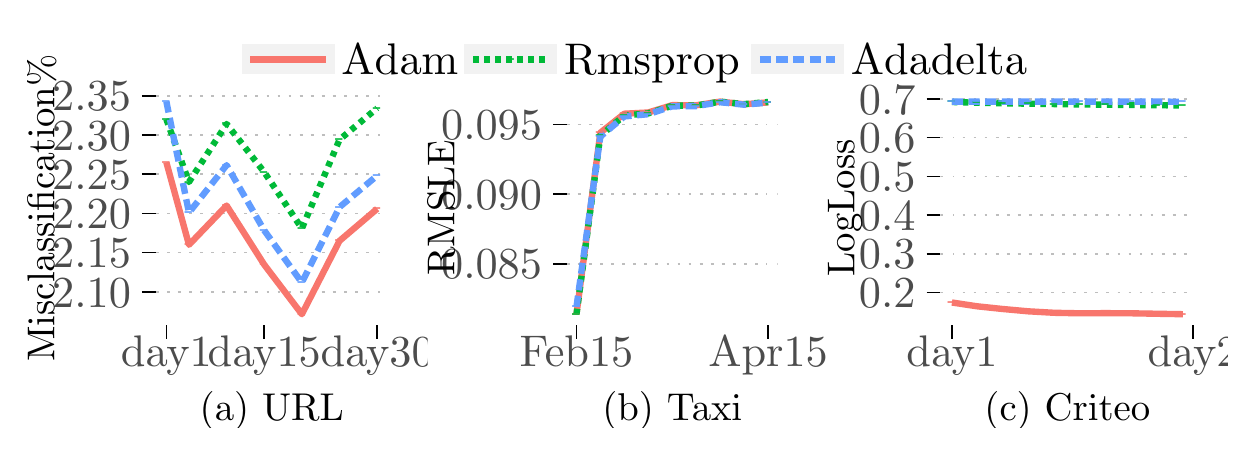
\begin{tikzpicture}[x=1pt,y=1pt]
\definecolor{fillColor}{RGB}{255,255,255}
\path[use as bounding box,fill=fillColor,fill opacity=0.00] (0,0) rectangle (433.62,144.54);
\begin{scope}
\path[clip] (  0.00,  0.00) rectangle (433.62,144.54);
\definecolor{fillColor}{RGB}{255,255,255}

\path[fill=fillColor] ( 67.06,121.66) rectangle (366.56,144.54);
\end{scope}
\begin{scope}
\path[clip] (  0.00,  0.00) rectangle (433.62,144.54);
\definecolor{drawColor}{RGB}{0,0,0}

\node[text=drawColor,anchor=base west,inner sep=0pt, outer sep=0pt, scale=  0.00] at ( 72.75,133.10) {Adaptation};
\end{scope}
\begin{scope}
\path[clip] (  0.00,  0.00) rectangle (433.62,144.54);
\definecolor{drawColor}{RGB}{255,255,255}
\definecolor{fillColor}{gray}{0.95}

\path[draw=drawColor,line width= 0.6pt,line join=round,line cap=round,fill=fillColor] ( 77.09,127.35) rectangle (111.23,138.85);
\end{scope}
\begin{scope}
\path[clip] (  0.00,  0.00) rectangle (433.62,144.54);
\definecolor{drawColor}{RGB}{248,118,109}

\path[draw=drawColor,line width= 2.3pt,line join=round] ( 80.51,133.10) -- (107.82,133.10);
\end{scope}
\begin{scope}
\path[clip] (  0.00,  0.00) rectangle (433.62,144.54);
\definecolor{drawColor}{RGB}{248,118,109}

\node[text=drawColor,anchor=base,inner sep=0pt, outer sep=0pt, scale=  1.00] at ( 94.16,130.94) {-};
\end{scope}
\begin{scope}
\path[clip] (  0.00,  0.00) rectangle (433.62,144.54);
\definecolor{drawColor}{RGB}{255,255,255}
\definecolor{fillColor}{gray}{0.95}

\path[draw=drawColor,line width= 0.6pt,line join=round,line cap=round,fill=fillColor] (157.52,127.35) rectangle (191.67,138.85);
\end{scope}
\begin{scope}
\path[clip] (  0.00,  0.00) rectangle (433.62,144.54);
\definecolor{drawColor}{RGB}{0,186,56}

\path[draw=drawColor,line width= 2.3pt,dash pattern=on 2pt off 2pt ,line join=round] (160.94,133.10) -- (188.25,133.10);
\end{scope}
\begin{scope}
\path[clip] (  0.00,  0.00) rectangle (433.62,144.54);
\definecolor{drawColor}{RGB}{0,186,56}

\node[text=drawColor,anchor=base,inner sep=0pt, outer sep=0pt, scale=  1.00] at (174.60,130.94) {-};
\end{scope}
\begin{scope}
\path[clip] (  0.00,  0.00) rectangle (433.62,144.54);
\definecolor{drawColor}{RGB}{255,255,255}
\definecolor{fillColor}{gray}{0.95}

\path[draw=drawColor,line width= 0.6pt,line join=round,line cap=round,fill=fillColor] (261.15,127.35) rectangle (295.30,138.85);
\end{scope}
\begin{scope}
\path[clip] (  0.00,  0.00) rectangle (433.62,144.54);
\definecolor{drawColor}{RGB}{97,156,255}

\path[draw=drawColor,line width= 2.3pt,dash pattern=on 4pt off 2pt ,line join=round] (264.57,133.10) -- (291.88,133.10);
\end{scope}
\begin{scope}
\path[clip] (  0.00,  0.00) rectangle (433.62,144.54);
\definecolor{drawColor}{RGB}{97,156,255}

\node[text=drawColor,anchor=base,inner sep=0pt, outer sep=0pt, scale=  1.00] at (278.22,130.94) {-};
\end{scope}
\begin{scope}
\path[clip] (  0.00,  0.00) rectangle (433.62,144.54);
\definecolor{drawColor}{RGB}{0,0,0}

\node[text=drawColor,anchor=base west,inner sep=0pt, outer sep=0pt, scale=  1.60] at (113.40,127.59) {Adam};
\end{scope}
\begin{scope}
\path[clip] (  0.00,  0.00) rectangle (433.62,144.54);
\definecolor{drawColor}{RGB}{0,0,0}

\node[text=drawColor,anchor=base west,inner sep=0pt, outer sep=0pt, scale=  1.60] at (193.84,127.59) {Rmsprop};
\end{scope}
\begin{scope}
\path[clip] (  0.00,  0.00) rectangle (433.62,144.54);
\definecolor{drawColor}{RGB}{0,0,0}

\node[text=drawColor,anchor=base west,inner sep=0pt, outer sep=0pt, scale=  1.60] at (297.46,127.59) {Adadelta};
\end{scope}
\begin{scope}
\path[clip] (  0.00,  0.00) rectangle (144.54,121.66);
\definecolor{drawColor}{RGB}{255,255,255}
\definecolor{fillColor}{RGB}{255,255,255}

\path[draw=drawColor,line width= 0.6pt,line join=round,line cap=round,fill=fillColor] (  0.00,  0.00) rectangle (144.54,121.66);
\end{scope}
\begin{scope}
\path[clip] ( 46.31, 37.15) rectangle (130.09,121.66);
\definecolor{fillColor}{RGB}{255,255,255}

\path[fill=fillColor] ( 46.31, 37.15) rectangle (130.09,121.66);
\definecolor{drawColor}{RGB}{255,255,255}

\path[draw=drawColor,line width= 0.3pt,line join=round] ( 46.31, 41.99) --
	(130.09, 41.99);

\path[draw=drawColor,line width= 0.3pt,line join=round] ( 46.31, 56.16) --
	(130.09, 56.16);

\path[draw=drawColor,line width= 0.3pt,line join=round] ( 46.31, 70.34) --
	(130.09, 70.34);

\path[draw=drawColor,line width= 0.3pt,line join=round] ( 46.31, 84.51) --
	(130.09, 84.51);

\path[draw=drawColor,line width= 0.3pt,line join=round] ( 46.31, 98.69) --
	(130.09, 98.69);

\path[draw=drawColor,line width= 0.3pt,line join=round] ( 46.31,112.86) --
	(130.09,112.86);

\path[draw=drawColor,line width= 0.3pt,line join=round] ( 67.80, 37.15) --
	( 67.80,121.66);

\path[draw=drawColor,line width= 0.3pt,line join=round] (105.88, 37.15) --
	(105.88,121.66);
\definecolor{drawColor}{RGB}{190,190,190}

\path[draw=drawColor,line width= 0.6pt,dash pattern=on 1pt off 3pt ,line join=round] ( 46.31, 49.08) --
	(130.09, 49.08);

\path[draw=drawColor,line width= 0.6pt,dash pattern=on 1pt off 3pt ,line join=round] ( 46.31, 63.25) --
	(130.09, 63.25);

\path[draw=drawColor,line width= 0.6pt,dash pattern=on 1pt off 3pt ,line join=round] ( 46.31, 77.42) --
	(130.09, 77.42);

\path[draw=drawColor,line width= 0.6pt,dash pattern=on 1pt off 3pt ,line join=round] ( 46.31, 91.60) --
	(130.09, 91.60);

\path[draw=drawColor,line width= 0.6pt,dash pattern=on 1pt off 3pt ,line join=round] ( 46.31,105.77) --
	(130.09,105.77);

\path[draw=drawColor,line width= 0.6pt,dash pattern=on 1pt off 3pt ,line join=round] ( 46.31,119.95) --
	(130.09,119.95);
\definecolor{drawColor}{RGB}{255,255,255}

\path[draw=drawColor,line width= 0.6pt,line join=round] ( 50.12, 37.15) --
	( 50.12,121.66);

\path[draw=drawColor,line width= 0.6pt,line join=round] ( 85.48, 37.15) --
	( 85.48,121.66);

\path[draw=drawColor,line width= 0.6pt,line join=round] (126.28, 37.15) --
	(126.28,121.66);
\definecolor{drawColor}{RGB}{248,118,109}

\path[draw=drawColor,line width= 2.3pt,line join=round] ( 50.12, 95.85) --
	( 58.28, 66.08) --
	( 71.88, 80.26) --
	( 85.48, 58.90) --
	( 99.08, 41.00) --
	(112.68, 67.50) --
	(126.28, 79.08);
\definecolor{drawColor}{RGB}{0,186,56}

\path[draw=drawColor,line width= 2.3pt,dash pattern=on 2pt off 2pt ,line join=round] ( 50.12,111.44) --
	( 58.28, 88.76) --
	( 71.88,109.74) --
	( 85.48, 92.35) --
	( 99.08, 71.97) --
	(112.68,104.07) --
	(126.28,115.46);
\definecolor{drawColor}{RGB}{97,156,255}

\path[draw=drawColor,line width= 2.3pt,dash pattern=on 4pt off 2pt ,line join=round] ( 50.12,117.82) --
	( 58.28, 77.71) --
	( 71.88, 94.86) --
	( 85.48, 71.28) --
	( 99.08, 52.41) --
	(112.68, 79.69) --
	(126.28, 91.08);
\definecolor{drawColor}{RGB}{248,118,109}

\node[text=drawColor,anchor=base,inner sep=0pt, outer sep=0pt, scale=  1.00] at ( 50.12, 93.69) {-};

\node[text=drawColor,anchor=base,inner sep=0pt, outer sep=0pt, scale=  1.00] at ( 58.28, 63.92) {-};

\node[text=drawColor,anchor=base,inner sep=0pt, outer sep=0pt, scale=  1.00] at ( 71.88, 78.10) {-};

\node[text=drawColor,anchor=base,inner sep=0pt, outer sep=0pt, scale=  1.00] at ( 85.48, 56.74) {-};

\node[text=drawColor,anchor=base,inner sep=0pt, outer sep=0pt, scale=  1.00] at ( 99.08, 38.83) {-};

\node[text=drawColor,anchor=base,inner sep=0pt, outer sep=0pt, scale=  1.00] at (112.68, 65.34) {-};

\node[text=drawColor,anchor=base,inner sep=0pt, outer sep=0pt, scale=  1.00] at (126.28, 76.92) {-};
\definecolor{drawColor}{RGB}{0,186,56}

\node[text=drawColor,anchor=base,inner sep=0pt, outer sep=0pt, scale=  1.00] at ( 50.12,109.28) {-};

\node[text=drawColor,anchor=base,inner sep=0pt, outer sep=0pt, scale=  1.00] at ( 58.28, 86.60) {-};

\node[text=drawColor,anchor=base,inner sep=0pt, outer sep=0pt, scale=  1.00] at ( 71.88,107.58) {-};

\node[text=drawColor,anchor=base,inner sep=0pt, outer sep=0pt, scale=  1.00] at ( 85.48, 90.19) {-};

\node[text=drawColor,anchor=base,inner sep=0pt, outer sep=0pt, scale=  1.00] at ( 99.08, 69.80) {-};

\node[text=drawColor,anchor=base,inner sep=0pt, outer sep=0pt, scale=  1.00] at (112.68,101.91) {-};

\node[text=drawColor,anchor=base,inner sep=0pt, outer sep=0pt, scale=  1.00] at (126.28,113.30) {-};
\definecolor{drawColor}{RGB}{97,156,255}

\node[text=drawColor,anchor=base,inner sep=0pt, outer sep=0pt, scale=  1.00] at ( 50.12,115.66) {-};

\node[text=drawColor,anchor=base,inner sep=0pt, outer sep=0pt, scale=  1.00] at ( 58.28, 75.54) {-};

\node[text=drawColor,anchor=base,inner sep=0pt, outer sep=0pt, scale=  1.00] at ( 71.88, 92.70) {-};

\node[text=drawColor,anchor=base,inner sep=0pt, outer sep=0pt, scale=  1.00] at ( 85.48, 69.12) {-};

\node[text=drawColor,anchor=base,inner sep=0pt, outer sep=0pt, scale=  1.00] at ( 99.08, 50.24) {-};

\node[text=drawColor,anchor=base,inner sep=0pt, outer sep=0pt, scale=  1.00] at (112.68, 77.53) {-};

\node[text=drawColor,anchor=base,inner sep=0pt, outer sep=0pt, scale=  1.00] at (126.28, 88.92) {-};
\end{scope}
\begin{scope}
\path[clip] (  0.00,  0.00) rectangle (433.62,144.54);
\definecolor{drawColor}{gray}{0.30}

\node[text=drawColor,anchor=base east,inner sep=0pt, outer sep=0pt, scale=  1.60] at ( 37.31, 43.57) {2.10};

\node[text=drawColor,anchor=base east,inner sep=0pt, outer sep=0pt, scale=  1.60] at ( 37.31, 57.74) {2.15};

\node[text=drawColor,anchor=base east,inner sep=0pt, outer sep=0pt, scale=  1.60] at ( 37.31, 71.91) {2.20};

\node[text=drawColor,anchor=base east,inner sep=0pt, outer sep=0pt, scale=  1.60] at ( 37.31, 86.09) {2.25};

\node[text=drawColor,anchor=base east,inner sep=0pt, outer sep=0pt, scale=  1.60] at ( 37.31,100.26) {2.30};

\node[text=drawColor,anchor=base east,inner sep=0pt, outer sep=0pt, scale=  1.60] at ( 37.31,114.44) {2.35};
\end{scope}
\begin{scope}
\path[clip] (  0.00,  0.00) rectangle (433.62,144.54);
\definecolor{drawColor}{RGB}{0,0,0}

\path[draw=drawColor,line width= 0.6pt,line join=round] ( 41.31, 49.08) --
	( 46.31, 49.08);

\path[draw=drawColor,line width= 0.6pt,line join=round] ( 41.31, 63.25) --
	( 46.31, 63.25);

\path[draw=drawColor,line width= 0.6pt,line join=round] ( 41.31, 77.42) --
	( 46.31, 77.42);

\path[draw=drawColor,line width= 0.6pt,line join=round] ( 41.31, 91.60) --
	( 46.31, 91.60);

\path[draw=drawColor,line width= 0.6pt,line join=round] ( 41.31,105.77) --
	( 46.31,105.77);

\path[draw=drawColor,line width= 0.6pt,line join=round] ( 41.31,119.95) --
	( 46.31,119.95);
\end{scope}
\begin{scope}
\path[clip] (  0.00,  0.00) rectangle (433.62,144.54);
\definecolor{drawColor}{RGB}{0,0,0}

\path[draw=drawColor,line width= 0.6pt,line join=round] ( 50.12, 32.15) --
	( 50.12, 37.15);

\path[draw=drawColor,line width= 0.6pt,line join=round] ( 85.48, 32.15) --
	( 85.48, 37.15);

\path[draw=drawColor,line width= 0.6pt,line join=round] (126.28, 32.15) --
	(126.28, 37.15);
\end{scope}
\begin{scope}
\path[clip] (  0.00,  0.00) rectangle (433.62,144.54);
\definecolor{drawColor}{gray}{0.30}

\node[text=drawColor,anchor=base,inner sep=0pt, outer sep=0pt, scale=  1.60] at ( 50.12, 22.14) {day1};

\node[text=drawColor,anchor=base,inner sep=0pt, outer sep=0pt, scale=  1.60] at ( 85.48, 22.14) {day15};

\node[text=drawColor,anchor=base,inner sep=0pt, outer sep=0pt, scale=  1.60] at (126.28, 22.14) {day30};
\end{scope}
\begin{scope}
\path[clip] (  0.00,  0.00) rectangle (433.62,144.54);
\definecolor{drawColor}{RGB}{0,0,0}

\node[text=drawColor,anchor=base,inner sep=0pt, outer sep=0pt, scale=  1.40] at ( 88.20,  2.49) {(a) URL};
\end{scope}
\begin{scope}
\path[clip] (  0.00,  0.00) rectangle (433.62,144.54);
\definecolor{drawColor}{RGB}{0,0,0}

\node[text=drawColor,rotate= 90.00,anchor=base,inner sep=0pt, outer sep=0pt, scale=  1.40] at (  9.64, 79.41) {Misclassification\%};
\end{scope}
\begin{scope}
\path[clip] (144.54,  0.00) rectangle (289.08,121.66);
\definecolor{drawColor}{RGB}{255,255,255}
\definecolor{fillColor}{RGB}{255,255,255}

\path[draw=drawColor,line width= 0.6pt,line join=round,line cap=round,fill=fillColor] (144.54,  0.00) rectangle (289.08,121.66);
\end{scope}
\begin{scope}
\path[clip] (194.85, 37.15) rectangle (271.01,121.66);
\definecolor{fillColor}{RGB}{255,255,255}

\path[fill=fillColor] (194.85, 37.15) rectangle (271.01,121.66);
\definecolor{drawColor}{RGB}{255,255,255}

\path[draw=drawColor,line width= 0.3pt,line join=round] (194.85, 46.69) --
	(271.01, 46.69);

\path[draw=drawColor,line width= 0.3pt,line join=round] (194.85, 71.81) --
	(271.01, 71.81);

\path[draw=drawColor,line width= 0.3pt,line join=round] (194.85, 96.93) --
	(271.01, 96.93);

\path[draw=drawColor,line width= 0.3pt,line join=round] (232.93, 37.15) --
	(232.93,121.66);
\definecolor{drawColor}{RGB}{190,190,190}

\path[draw=drawColor,line width= 0.6pt,dash pattern=on 1pt off 3pt ,line join=round] (194.85, 59.25) --
	(271.01, 59.25);

\path[draw=drawColor,line width= 0.6pt,dash pattern=on 1pt off 3pt ,line join=round] (194.85, 84.37) --
	(271.01, 84.37);

\path[draw=drawColor,line width= 0.6pt,dash pattern=on 1pt off 3pt ,line join=round] (194.85,109.49) --
	(271.01,109.49);
\definecolor{drawColor}{RGB}{255,255,255}

\path[draw=drawColor,line width= 0.6pt,line join=round] (198.31, 37.15) --
	(198.31,121.66);

\path[draw=drawColor,line width= 0.6pt,line join=round] (267.55, 37.15) --
	(267.55,121.66);
\definecolor{drawColor}{RGB}{248,118,109}

\path[draw=drawColor,line width= 2.3pt,line join=round] (198.31, 41.06) --
	(206.93,106.58) --
	(215.59,113.45) --
	(224.25,113.89) --
	(232.91,116.54) --
	(241.57,116.50) --
	(250.23,117.82) --
	(258.89,116.86) --
	(267.55,117.55);
\definecolor{drawColor}{RGB}{0,186,56}

\path[draw=drawColor,line width= 2.3pt,dash pattern=on 2pt off 2pt ,line join=round] (198.31, 41.00) --
	(206.93,105.43) --
	(215.59,112.82) --
	(224.25,113.56) --
	(232.91,116.33) --
	(241.57,116.39) --
	(250.23,117.80) --
	(258.89,116.91) --
	(267.55,117.68);
\definecolor{drawColor}{RGB}{97,156,255}

\path[draw=drawColor,line width= 2.3pt,dash pattern=on 4pt off 2pt ,line join=round] (198.31, 43.71) --
	(206.93,105.17) --
	(215.59,112.46) --
	(224.25,113.27) --
	(232.91,116.10) --
	(241.57,116.20) --
	(250.23,117.60) --
	(258.89,116.71) --
	(267.55,117.46);
\definecolor{drawColor}{RGB}{248,118,109}

\node[text=drawColor,anchor=base,inner sep=0pt, outer sep=0pt, scale=  1.00] at (198.31, 38.90) {-};

\node[text=drawColor,anchor=base,inner sep=0pt, outer sep=0pt, scale=  1.00] at (206.93,104.42) {-};

\node[text=drawColor,anchor=base,inner sep=0pt, outer sep=0pt, scale=  1.00] at (215.59,111.29) {-};

\node[text=drawColor,anchor=base,inner sep=0pt, outer sep=0pt, scale=  1.00] at (224.25,111.73) {-};

\node[text=drawColor,anchor=base,inner sep=0pt, outer sep=0pt, scale=  1.00] at (232.91,114.37) {-};

\node[text=drawColor,anchor=base,inner sep=0pt, outer sep=0pt, scale=  1.00] at (241.57,114.33) {-};

\node[text=drawColor,anchor=base,inner sep=0pt, outer sep=0pt, scale=  1.00] at (250.23,115.66) {-};

\node[text=drawColor,anchor=base,inner sep=0pt, outer sep=0pt, scale=  1.00] at (258.89,114.69) {-};

\node[text=drawColor,anchor=base,inner sep=0pt, outer sep=0pt, scale=  1.00] at (267.55,115.39) {-};
\definecolor{drawColor}{RGB}{0,186,56}

\node[text=drawColor,anchor=base,inner sep=0pt, outer sep=0pt, scale=  1.00] at (198.31, 38.83) {-};

\node[text=drawColor,anchor=base,inner sep=0pt, outer sep=0pt, scale=  1.00] at (206.93,103.26) {-};

\node[text=drawColor,anchor=base,inner sep=0pt, outer sep=0pt, scale=  1.00] at (215.59,110.66) {-};

\node[text=drawColor,anchor=base,inner sep=0pt, outer sep=0pt, scale=  1.00] at (224.25,111.40) {-};

\node[text=drawColor,anchor=base,inner sep=0pt, outer sep=0pt, scale=  1.00] at (232.91,114.17) {-};

\node[text=drawColor,anchor=base,inner sep=0pt, outer sep=0pt, scale=  1.00] at (241.57,114.23) {-};

\node[text=drawColor,anchor=base,inner sep=0pt, outer sep=0pt, scale=  1.00] at (250.23,115.63) {-};

\node[text=drawColor,anchor=base,inner sep=0pt, outer sep=0pt, scale=  1.00] at (258.89,114.74) {-};

\node[text=drawColor,anchor=base,inner sep=0pt, outer sep=0pt, scale=  1.00] at (267.55,115.51) {-};
\definecolor{drawColor}{RGB}{97,156,255}

\node[text=drawColor,anchor=base,inner sep=0pt, outer sep=0pt, scale=  1.00] at (198.31, 41.54) {-};

\node[text=drawColor,anchor=base,inner sep=0pt, outer sep=0pt, scale=  1.00] at (206.93,103.01) {-};

\node[text=drawColor,anchor=base,inner sep=0pt, outer sep=0pt, scale=  1.00] at (215.59,110.30) {-};

\node[text=drawColor,anchor=base,inner sep=0pt, outer sep=0pt, scale=  1.00] at (224.25,111.10) {-};

\node[text=drawColor,anchor=base,inner sep=0pt, outer sep=0pt, scale=  1.00] at (232.91,113.94) {-};

\node[text=drawColor,anchor=base,inner sep=0pt, outer sep=0pt, scale=  1.00] at (241.57,114.04) {-};

\node[text=drawColor,anchor=base,inner sep=0pt, outer sep=0pt, scale=  1.00] at (250.23,115.43) {-};

\node[text=drawColor,anchor=base,inner sep=0pt, outer sep=0pt, scale=  1.00] at (258.89,114.55) {-};

\node[text=drawColor,anchor=base,inner sep=0pt, outer sep=0pt, scale=  1.00] at (267.55,115.30) {-};
\end{scope}
\begin{scope}
\path[clip] (  0.00,  0.00) rectangle (433.62,144.54);
\definecolor{drawColor}{gray}{0.30}

\node[text=drawColor,anchor=base east,inner sep=0pt, outer sep=0pt, scale=  1.60] at (185.85, 53.74) {0.085};

\node[text=drawColor,anchor=base east,inner sep=0pt, outer sep=0pt, scale=  1.60] at (185.85, 78.86) {0.090};

\node[text=drawColor,anchor=base east,inner sep=0pt, outer sep=0pt, scale=  1.60] at (185.85,103.98) {0.095};
\end{scope}
\begin{scope}
\path[clip] (  0.00,  0.00) rectangle (433.62,144.54);
\definecolor{drawColor}{RGB}{0,0,0}

\path[draw=drawColor,line width= 0.6pt,line join=round] (189.85, 59.25) --
	(194.85, 59.25);

\path[draw=drawColor,line width= 0.6pt,line join=round] (189.85, 84.37) --
	(194.85, 84.37);

\path[draw=drawColor,line width= 0.6pt,line join=round] (189.85,109.49) --
	(194.85,109.49);
\end{scope}
\begin{scope}
\path[clip] (  0.00,  0.00) rectangle (433.62,144.54);
\definecolor{drawColor}{RGB}{0,0,0}

\path[draw=drawColor,line width= 0.6pt,line join=round] (198.31, 32.15) --
	(198.31, 37.15);

\path[draw=drawColor,line width= 0.6pt,line join=round] (267.55, 32.15) --
	(267.55, 37.15);
\end{scope}
\begin{scope}
\path[clip] (  0.00,  0.00) rectangle (433.62,144.54);
\definecolor{drawColor}{gray}{0.30}

\node[text=drawColor,anchor=base,inner sep=0pt, outer sep=0pt, scale=  1.60] at (198.31, 22.14) {Feb15};

\node[text=drawColor,anchor=base,inner sep=0pt, outer sep=0pt, scale=  1.60] at (267.55, 22.14) {Apr15};
\end{scope}
\begin{scope}
\path[clip] (  0.00,  0.00) rectangle (433.62,144.54);
\definecolor{drawColor}{RGB}{0,0,0}

\node[text=drawColor,anchor=base,inner sep=0pt, outer sep=0pt, scale=  1.40] at (232.93,  2.49) {(b) Taxi};
\end{scope}
\begin{scope}
\path[clip] (  0.00,  0.00) rectangle (433.62,144.54);
\definecolor{drawColor}{RGB}{0,0,0}

\node[text=drawColor,rotate= 90.00,anchor=base,inner sep=0pt, outer sep=0pt, scale=  1.40] at (154.18, 79.41) {RMSLE};
\end{scope}
\begin{scope}
\path[clip] (289.08,  0.00) rectangle (433.62,121.66);
\definecolor{drawColor}{RGB}{255,255,255}
\definecolor{fillColor}{RGB}{255,255,255}

\path[draw=drawColor,line width= 0.6pt,line join=round,line cap=round,fill=fillColor] (289.08,  0.00) rectangle (433.62,121.66);
\end{scope}
\begin{scope}
\path[clip] (329.81, 37.15) rectangle (421.57,121.66);
\definecolor{fillColor}{RGB}{255,255,255}

\path[fill=fillColor] (329.81, 37.15) rectangle (421.57,121.66);
\definecolor{drawColor}{RGB}{255,255,255}

\path[draw=drawColor,line width= 0.3pt,line join=round] (329.81, 41.88) --
	(421.57, 41.88);

\path[draw=drawColor,line width= 0.3pt,line join=round] (329.81, 55.86) --
	(421.57, 55.86);

\path[draw=drawColor,line width= 0.3pt,line join=round] (329.81, 69.84) --
	(421.57, 69.84);

\path[draw=drawColor,line width= 0.3pt,line join=round] (329.81, 83.83) --
	(421.57, 83.83);

\path[draw=drawColor,line width= 0.3pt,line join=round] (329.81, 97.81) --
	(421.57, 97.81);

\path[draw=drawColor,line width= 0.3pt,line join=round] (329.81,111.79) --
	(421.57,111.79);

\path[draw=drawColor,line width= 0.3pt,line join=round] (377.55, 37.15) --
	(377.55,121.66);
\definecolor{drawColor}{RGB}{190,190,190}

\path[draw=drawColor,line width= 0.6pt,dash pattern=on 1pt off 3pt ,line join=round] (329.81, 48.87) --
	(421.57, 48.87);

\path[draw=drawColor,line width= 0.6pt,dash pattern=on 1pt off 3pt ,line join=round] (329.81, 62.85) --
	(421.57, 62.85);

\path[draw=drawColor,line width= 0.6pt,dash pattern=on 1pt off 3pt ,line join=round] (329.81, 76.83) --
	(421.57, 76.83);

\path[draw=drawColor,line width= 0.6pt,dash pattern=on 1pt off 3pt ,line join=round] (329.81, 90.82) --
	(421.57, 90.82);

\path[draw=drawColor,line width= 0.6pt,dash pattern=on 1pt off 3pt ,line join=round] (329.81,104.80) --
	(421.57,104.80);

\path[draw=drawColor,line width= 0.6pt,dash pattern=on 1pt off 3pt ,line join=round] (329.81,118.78) --
	(421.57,118.78);
\definecolor{drawColor}{RGB}{255,255,255}

\path[draw=drawColor,line width= 0.6pt,line join=round] (333.98, 37.15) --
	(333.98,121.66);

\path[draw=drawColor,line width= 0.6pt,line join=round] (421.12, 37.15) --
	(421.12,121.66);
\definecolor{drawColor}{RGB}{248,118,109}

\path[draw=drawColor,line width= 2.3pt,line join=round] (333.98, 45.23) --
	(343.05, 43.86) --
	(352.34, 42.88) --
	(361.63, 42.04) --
	(370.93, 41.51) --
	(380.22, 41.33) --
	(389.52, 41.38) --
	(398.81, 41.33) --
	(408.11, 41.16) --
	(417.40, 41.00);
\definecolor{drawColor}{RGB}{0,186,56}

\path[draw=drawColor,line width= 2.3pt,dash pattern=on 2pt off 2pt ,line join=round] (333.98,117.68) --
	(343.05,117.43) --
	(352.34,117.23) --
	(361.63,117.07) --
	(370.93,116.93) --
	(380.22,116.80) --
	(389.52,116.70) --
	(398.81,116.60) --
	(408.11,116.51) --
	(417.40,116.43);
\definecolor{drawColor}{RGB}{97,156,255}

\path[draw=drawColor,line width= 2.3pt,dash pattern=on 4pt off 2pt ,line join=round] (333.98,117.82) --
	(343.05,117.82) --
	(352.34,117.82) --
	(361.63,117.81) --
	(370.93,117.81) --
	(380.22,117.81) --
	(389.52,117.80) --
	(398.81,117.80) --
	(408.11,117.80) --
	(417.40,117.79);
\definecolor{drawColor}{RGB}{248,118,109}

\node[text=drawColor,anchor=base,inner sep=0pt, outer sep=0pt, scale=  1.00] at (333.98, 43.07) {-};

\node[text=drawColor,anchor=base,inner sep=0pt, outer sep=0pt, scale=  1.00] at (343.05, 41.70) {-};

\node[text=drawColor,anchor=base,inner sep=0pt, outer sep=0pt, scale=  1.00] at (352.34, 40.72) {-};

\node[text=drawColor,anchor=base,inner sep=0pt, outer sep=0pt, scale=  1.00] at (361.63, 39.88) {-};

\node[text=drawColor,anchor=base,inner sep=0pt, outer sep=0pt, scale=  1.00] at (370.93, 39.34) {-};

\node[text=drawColor,anchor=base,inner sep=0pt, outer sep=0pt, scale=  1.00] at (380.22, 39.16) {-};

\node[text=drawColor,anchor=base,inner sep=0pt, outer sep=0pt, scale=  1.00] at (389.52, 39.22) {-};

\node[text=drawColor,anchor=base,inner sep=0pt, outer sep=0pt, scale=  1.00] at (398.81, 39.16) {-};

\node[text=drawColor,anchor=base,inner sep=0pt, outer sep=0pt, scale=  1.00] at (408.11, 38.99) {-};

\node[text=drawColor,anchor=base,inner sep=0pt, outer sep=0pt, scale=  1.00] at (417.40, 38.83) {-};
\definecolor{drawColor}{RGB}{0,186,56}

\node[text=drawColor,anchor=base,inner sep=0pt, outer sep=0pt, scale=  1.00] at (333.98,115.52) {-};

\node[text=drawColor,anchor=base,inner sep=0pt, outer sep=0pt, scale=  1.00] at (343.05,115.27) {-};

\node[text=drawColor,anchor=base,inner sep=0pt, outer sep=0pt, scale=  1.00] at (352.34,115.07) {-};

\node[text=drawColor,anchor=base,inner sep=0pt, outer sep=0pt, scale=  1.00] at (361.63,114.91) {-};

\node[text=drawColor,anchor=base,inner sep=0pt, outer sep=0pt, scale=  1.00] at (370.93,114.76) {-};

\node[text=drawColor,anchor=base,inner sep=0pt, outer sep=0pt, scale=  1.00] at (380.22,114.64) {-};

\node[text=drawColor,anchor=base,inner sep=0pt, outer sep=0pt, scale=  1.00] at (389.52,114.53) {-};

\node[text=drawColor,anchor=base,inner sep=0pt, outer sep=0pt, scale=  1.00] at (398.81,114.44) {-};

\node[text=drawColor,anchor=base,inner sep=0pt, outer sep=0pt, scale=  1.00] at (408.11,114.35) {-};

\node[text=drawColor,anchor=base,inner sep=0pt, outer sep=0pt, scale=  1.00] at (417.40,114.27) {-};
\definecolor{drawColor}{RGB}{97,156,255}

\node[text=drawColor,anchor=base,inner sep=0pt, outer sep=0pt, scale=  1.00] at (333.98,115.66) {-};

\node[text=drawColor,anchor=base,inner sep=0pt, outer sep=0pt, scale=  1.00] at (343.05,115.66) {-};

\node[text=drawColor,anchor=base,inner sep=0pt, outer sep=0pt, scale=  1.00] at (352.34,115.65) {-};

\node[text=drawColor,anchor=base,inner sep=0pt, outer sep=0pt, scale=  1.00] at (361.63,115.65) {-};

\node[text=drawColor,anchor=base,inner sep=0pt, outer sep=0pt, scale=  1.00] at (370.93,115.65) {-};

\node[text=drawColor,anchor=base,inner sep=0pt, outer sep=0pt, scale=  1.00] at (380.22,115.64) {-};

\node[text=drawColor,anchor=base,inner sep=0pt, outer sep=0pt, scale=  1.00] at (389.52,115.64) {-};

\node[text=drawColor,anchor=base,inner sep=0pt, outer sep=0pt, scale=  1.00] at (398.81,115.64) {-};

\node[text=drawColor,anchor=base,inner sep=0pt, outer sep=0pt, scale=  1.00] at (408.11,115.63) {-};

\node[text=drawColor,anchor=base,inner sep=0pt, outer sep=0pt, scale=  1.00] at (417.40,115.63) {-};
\end{scope}
\begin{scope}
\path[clip] (  0.00,  0.00) rectangle (433.62,144.54);
\definecolor{drawColor}{gray}{0.30}

\node[text=drawColor,anchor=base east,inner sep=0pt, outer sep=0pt, scale=  1.60] at (320.81, 43.36) {0.2};

\node[text=drawColor,anchor=base east,inner sep=0pt, outer sep=0pt, scale=  1.60] at (320.81, 57.34) {0.3};

\node[text=drawColor,anchor=base east,inner sep=0pt, outer sep=0pt, scale=  1.60] at (320.81, 71.32) {0.4};

\node[text=drawColor,anchor=base east,inner sep=0pt, outer sep=0pt, scale=  1.60] at (320.81, 85.31) {0.5};

\node[text=drawColor,anchor=base east,inner sep=0pt, outer sep=0pt, scale=  1.60] at (320.81, 99.29) {0.6};

\node[text=drawColor,anchor=base east,inner sep=0pt, outer sep=0pt, scale=  1.60] at (320.81,113.27) {0.7};
\end{scope}
\begin{scope}
\path[clip] (  0.00,  0.00) rectangle (433.62,144.54);
\definecolor{drawColor}{RGB}{0,0,0}

\path[draw=drawColor,line width= 0.6pt,line join=round] (324.81, 48.87) --
	(329.81, 48.87);

\path[draw=drawColor,line width= 0.6pt,line join=round] (324.81, 62.85) --
	(329.81, 62.85);

\path[draw=drawColor,line width= 0.6pt,line join=round] (324.81, 76.83) --
	(329.81, 76.83);

\path[draw=drawColor,line width= 0.6pt,line join=round] (324.81, 90.82) --
	(329.81, 90.82);

\path[draw=drawColor,line width= 0.6pt,line join=round] (324.81,104.80) --
	(329.81,104.80);

\path[draw=drawColor,line width= 0.6pt,line join=round] (324.81,118.78) --
	(329.81,118.78);
\end{scope}
\begin{scope}
\path[clip] (  0.00,  0.00) rectangle (433.62,144.54);
\definecolor{drawColor}{RGB}{0,0,0}

\path[draw=drawColor,line width= 0.6pt,line join=round] (333.98, 32.15) --
	(333.98, 37.15);

\path[draw=drawColor,line width= 0.6pt,line join=round] (421.12, 32.15) --
	(421.12, 37.15);
\end{scope}
\begin{scope}
\path[clip] (  0.00,  0.00) rectangle (433.62,144.54);
\definecolor{drawColor}{gray}{0.30}

\node[text=drawColor,anchor=base,inner sep=0pt, outer sep=0pt, scale=  1.60] at (333.98, 22.14) {day1};

\node[text=drawColor,anchor=base,inner sep=0pt, outer sep=0pt, scale=  1.60] at (421.12, 22.14) {day2};
\end{scope}
\begin{scope}
\path[clip] (  0.00,  0.00) rectangle (433.62,144.54);
\definecolor{drawColor}{RGB}{0,0,0}

\node[text=drawColor,anchor=base,inner sep=0pt, outer sep=0pt, scale=  1.40] at (375.69,  2.49) {(c) Criteo};
\end{scope}
\begin{scope}
\path[clip] (  0.00,  0.00) rectangle (433.62,144.54);
\definecolor{drawColor}{RGB}{0,0,0}

\node[text=drawColor,rotate= 90.00,anchor=base,inner sep=0pt, outer sep=0pt, scale=  1.40] at (298.72, 79.41) {LogLoss};
\end{scope}
\end{tikzpicture}
}
\caption{Result of hyperparameter tuning during initial phases of deployment}
\label{hyper-param-figure}
\end{figure}

\textbf{Sampling Methods.}
The proactive training is also affected by the choice of the sampling method.
Each instance of the proactive training updates the deployed model using the provided sample.
Therefore, the quality of the model after an update is directly related to the quality of the data inside the sample.
We evaluate the effect of three different sampling methods, time-based, window-based, and uniform, on the quality of the deployed model.
The time-based sampling method is a weighted sampling approach that assigns higher weights to the recent items. 
The window-based sampling method only samples data from an active window, where the size of the window is 10\% of the total deployment duration (12 days for URL, 2 months for Taxi, and 1.5 days for Criteo).
Finally, uniform sampling method samples data from the entire previously seen data.
For each pipeline, the sampling rate for the proactive training is similar to the sampling rate of the initial stochastic gradient descent optimization(0.1 for all three pipelines).
Figure \ref{sampling-method-figure} shows the effect of different sampling methods on the quality of the model during the deployment phase.
\todo[inline]{I expect similar performance for taxi and criteo, therefore I will not talk about each figure individually}
Time-based sampling achieves the highest quality for all the models.
Every dataset is gathered throughout a long period of time.
Therefore, the underlying characteristics of the data gradually change over time.
A time-based sampling approach is more likely to select the recent items for the proactive training.
As a result, the deployed model is influenced by the more recent items and performs better on the incoming prediction requests.
For the URL pipeline, window-based and uniform sampling have very similar performances.

\begin{figure}[!h]
\centering
\resizebox{\columnwidth}{!}{% Created by tikzDevice version 0.11 on 2018-05-19 10:35:13
% !TEX encoding = UTF-8 Unicode
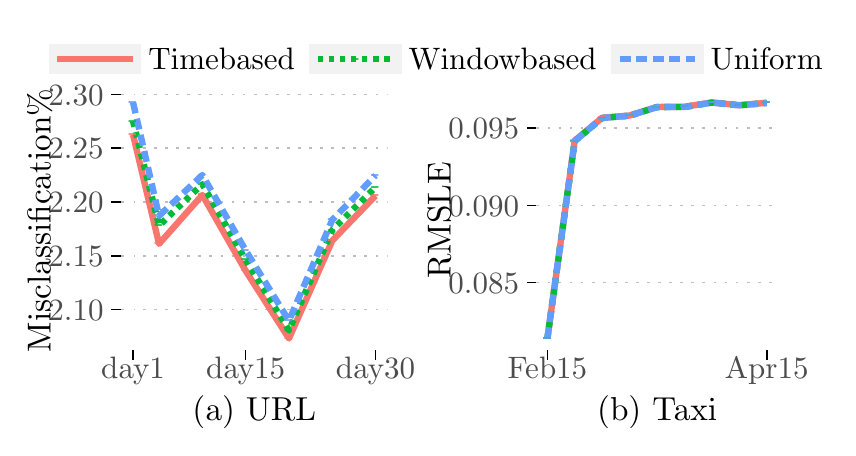
\begin{tikzpicture}[x=1pt,y=1pt]
\definecolor{fillColor}{RGB}{255,255,255}
\path[use as bounding box,fill=fillColor,fill opacity=0.00] (0,0) rectangle (289.08,144.54);
\begin{scope}
\path[clip] (  0.00,  0.00) rectangle (289.08,144.54);
\definecolor{fillColor}{RGB}{255,255,255}

\path[fill=fillColor] ( -2.74,121.78) rectangle (291.82,144.54);
\end{scope}
\begin{scope}
\path[clip] (  0.00,  0.00) rectangle (289.08,144.54);
\definecolor{drawColor}{RGB}{0,0,0}

\node[text=drawColor,anchor=base west,inner sep=0pt, outer sep=0pt, scale=  0.00] at (  2.95,133.16) {Sampling};
\end{scope}
\begin{scope}
\path[clip] (  0.00,  0.00) rectangle (289.08,144.54);
\definecolor{drawColor}{RGB}{255,255,255}
\definecolor{fillColor}{gray}{0.95}

\path[draw=drawColor,line width= 0.6pt,line join=round,line cap=round,fill=fillColor] (  7.28,127.47) rectangle ( 41.43,138.85);
\end{scope}
\begin{scope}
\path[clip] (  0.00,  0.00) rectangle (289.08,144.54);
\definecolor{drawColor}{RGB}{248,118,109}

\path[draw=drawColor,line width= 2.3pt,line join=round] ( 10.70,133.16) -- ( 38.01,133.16);
\end{scope}
\begin{scope}
\path[clip] (  0.00,  0.00) rectangle (289.08,144.54);
\definecolor{drawColor}{RGB}{248,118,109}

\node[text=drawColor,anchor=base,inner sep=0pt, outer sep=0pt, scale=  1.00] at ( 24.36,131.00) {-};
\end{scope}
\begin{scope}
\path[clip] (  0.00,  0.00) rectangle (289.08,144.54);
\definecolor{drawColor}{RGB}{255,255,255}
\definecolor{fillColor}{gray}{0.95}

\path[draw=drawColor,line width= 0.6pt,line join=round,line cap=round,fill=fillColor] (101.38,127.47) rectangle (135.52,138.85);
\end{scope}
\begin{scope}
\path[clip] (  0.00,  0.00) rectangle (289.08,144.54);
\definecolor{drawColor}{RGB}{0,186,56}

\path[draw=drawColor,line width= 2.3pt,dash pattern=on 2pt off 2pt ,line join=round] (104.79,133.16) -- (132.10,133.16);
\end{scope}
\begin{scope}
\path[clip] (  0.00,  0.00) rectangle (289.08,144.54);
\definecolor{drawColor}{RGB}{0,186,56}

\node[text=drawColor,anchor=base,inner sep=0pt, outer sep=0pt, scale=  1.00] at (118.45,131.00) {-};
\end{scope}
\begin{scope}
\path[clip] (  0.00,  0.00) rectangle (289.08,144.54);
\definecolor{drawColor}{RGB}{255,255,255}
\definecolor{fillColor}{gray}{0.95}

\path[draw=drawColor,line width= 0.6pt,line join=round,line cap=round,fill=fillColor] (210.47,127.47) rectangle (244.61,138.85);
\end{scope}
\begin{scope}
\path[clip] (  0.00,  0.00) rectangle (289.08,144.54);
\definecolor{drawColor}{RGB}{97,156,255}

\path[draw=drawColor,line width= 2.3pt,dash pattern=on 4pt off 2pt ,line join=round] (213.88,133.16) -- (241.20,133.16);
\end{scope}
\begin{scope}
\path[clip] (  0.00,  0.00) rectangle (289.08,144.54);
\definecolor{drawColor}{RGB}{97,156,255}

\node[text=drawColor,anchor=base,inner sep=0pt, outer sep=0pt, scale=  1.00] at (227.54,131.00) {-};
\end{scope}
\begin{scope}
\path[clip] (  0.00,  0.00) rectangle (289.08,144.54);
\definecolor{drawColor}{RGB}{0,0,0}

\node[text=drawColor,anchor=base west,inner sep=0pt, outer sep=0pt, scale=  1.12] at ( 43.60,129.30) {Timebased};
\end{scope}
\begin{scope}
\path[clip] (  0.00,  0.00) rectangle (289.08,144.54);
\definecolor{drawColor}{RGB}{0,0,0}

\node[text=drawColor,anchor=base west,inner sep=0pt, outer sep=0pt, scale=  1.12] at (137.69,129.30) {Windowbased};
\end{scope}
\begin{scope}
\path[clip] (  0.00,  0.00) rectangle (289.08,144.54);
\definecolor{drawColor}{RGB}{0,0,0}

\node[text=drawColor,anchor=base west,inner sep=0pt, outer sep=0pt, scale=  1.12] at (246.78,129.30) {Uniform};
\end{scope}
\begin{scope}
\path[clip] (  0.00,  0.00) rectangle (144.54,121.78);
\definecolor{drawColor}{RGB}{255,255,255}
\definecolor{fillColor}{RGB}{255,255,255}

\path[draw=drawColor,line width= 0.6pt,line join=round,line cap=round,fill=fillColor] ( -0.00,  0.00) rectangle (144.54,121.78);
\end{scope}
\begin{scope}
\path[clip] ( 33.70, 27.97) rectangle (130.09,121.78);
\definecolor{fillColor}{RGB}{255,255,255}

\path[fill=fillColor] ( 33.70, 27.97) rectangle (130.09,121.78);
\definecolor{drawColor}{RGB}{255,255,255}

\path[draw=drawColor,line width= 0.3pt,line join=round] ( 33.70, 33.01) --
	(130.09, 33.01);

\path[draw=drawColor,line width= 0.3pt,line join=round] ( 33.70, 52.44) --
	(130.09, 52.44);

\path[draw=drawColor,line width= 0.3pt,line join=round] ( 33.70, 71.86) --
	(130.09, 71.86);

\path[draw=drawColor,line width= 0.3pt,line join=round] ( 33.70, 91.29) --
	(130.09, 91.29);

\path[draw=drawColor,line width= 0.3pt,line join=round] ( 33.70,110.71) --
	(130.09,110.71);

\path[draw=drawColor,line width= 0.3pt,line join=round] ( 58.42, 27.97) --
	( 58.42,121.78);

\path[draw=drawColor,line width= 0.3pt,line join=round] (102.23, 27.97) --
	(102.23,121.78);
\definecolor{drawColor}{RGB}{190,190,190}

\path[draw=drawColor,line width= 0.6pt,dash pattern=on 1pt off 3pt ,line join=round] ( 33.70, 42.73) --
	(130.09, 42.73);

\path[draw=drawColor,line width= 0.6pt,dash pattern=on 1pt off 3pt ,line join=round] ( 33.70, 62.15) --
	(130.09, 62.15);

\path[draw=drawColor,line width= 0.6pt,dash pattern=on 1pt off 3pt ,line join=round] ( 33.70, 81.58) --
	(130.09, 81.58);

\path[draw=drawColor,line width= 0.6pt,dash pattern=on 1pt off 3pt ,line join=round] ( 33.70,101.00) --
	(130.09,101.00);

\path[draw=drawColor,line width= 0.6pt,dash pattern=on 1pt off 3pt ,line join=round] ( 33.70,120.43) --
	(130.09,120.43);
\definecolor{drawColor}{RGB}{255,255,255}

\path[draw=drawColor,line width= 0.6pt,line join=round] ( 38.08, 27.97) --
	( 38.08,121.78);

\path[draw=drawColor,line width= 0.6pt,line join=round] ( 78.76, 27.97) --
	( 78.76,121.78);

\path[draw=drawColor,line width= 0.6pt,line join=round] (125.70, 27.97) --
	(125.70,121.78);
\definecolor{drawColor}{RGB}{248,118,109}

\path[draw=drawColor,line width= 2.3pt,line join=round] ( 38.08,105.86) --
	( 47.47, 66.42) --
	( 63.12, 84.10) --
	( 78.76, 56.71) --
	( 94.41, 32.24) --
	(110.06, 67.59) --
	(125.70, 83.84);
\definecolor{drawColor}{RGB}{0,186,56}

\path[draw=drawColor,line width= 2.3pt,dash pattern=on 2pt off 2pt ,line join=round] ( 38.08,110.71) --
	( 47.47, 73.03) --
	( 63.12, 87.99) --
	( 78.76, 60.60) --
	( 94.41, 35.15) --
	(110.06, 71.40) --
	(125.70, 86.95);
\definecolor{drawColor}{RGB}{97,156,255}

\path[draw=drawColor,line width= 2.3pt,dash pattern=on 4pt off 2pt ,line join=round] ( 38.08,117.51) --
	( 47.47, 76.53) --
	( 63.12, 91.29) --
	( 78.76, 64.09) --
	( 94.41, 38.65) --
	(110.06, 75.05) --
	(125.70, 91.16);
\definecolor{drawColor}{RGB}{248,118,109}

\node[text=drawColor,anchor=base,inner sep=0pt, outer sep=0pt, scale=  1.00] at ( 38.08,103.70) {-};

\node[text=drawColor,anchor=base,inner sep=0pt, outer sep=0pt, scale=  1.00] at ( 47.47, 64.26) {-};

\node[text=drawColor,anchor=base,inner sep=0pt, outer sep=0pt, scale=  1.00] at ( 63.12, 81.94) {-};

\node[text=drawColor,anchor=base,inner sep=0pt, outer sep=0pt, scale=  1.00] at ( 78.76, 54.55) {-};

\node[text=drawColor,anchor=base,inner sep=0pt, outer sep=0pt, scale=  1.00] at ( 94.41, 30.07) {-};

\node[text=drawColor,anchor=base,inner sep=0pt, outer sep=0pt, scale=  1.00] at (110.06, 65.43) {-};

\node[text=drawColor,anchor=base,inner sep=0pt, outer sep=0pt, scale=  1.00] at (125.70, 81.68) {-};
\definecolor{drawColor}{RGB}{0,186,56}

\node[text=drawColor,anchor=base,inner sep=0pt, outer sep=0pt, scale=  1.00] at ( 38.08,108.55) {-};

\node[text=drawColor,anchor=base,inner sep=0pt, outer sep=0pt, scale=  1.00] at ( 47.47, 70.87) {-};

\node[text=drawColor,anchor=base,inner sep=0pt, outer sep=0pt, scale=  1.00] at ( 63.12, 85.82) {-};

\node[text=drawColor,anchor=base,inner sep=0pt, outer sep=0pt, scale=  1.00] at ( 78.76, 58.43) {-};

\node[text=drawColor,anchor=base,inner sep=0pt, outer sep=0pt, scale=  1.00] at ( 94.41, 32.99) {-};

\node[text=drawColor,anchor=base,inner sep=0pt, outer sep=0pt, scale=  1.00] at (110.06, 69.23) {-};

\node[text=drawColor,anchor=base,inner sep=0pt, outer sep=0pt, scale=  1.00] at (125.70, 84.79) {-};
\definecolor{drawColor}{RGB}{97,156,255}

\node[text=drawColor,anchor=base,inner sep=0pt, outer sep=0pt, scale=  1.00] at ( 38.08,115.35) {-};

\node[text=drawColor,anchor=base,inner sep=0pt, outer sep=0pt, scale=  1.00] at ( 47.47, 74.36) {-};

\node[text=drawColor,anchor=base,inner sep=0pt, outer sep=0pt, scale=  1.00] at ( 63.12, 89.13) {-};

\node[text=drawColor,anchor=base,inner sep=0pt, outer sep=0pt, scale=  1.00] at ( 78.76, 61.93) {-};

\node[text=drawColor,anchor=base,inner sep=0pt, outer sep=0pt, scale=  1.00] at ( 94.41, 36.48) {-};

\node[text=drawColor,anchor=base,inner sep=0pt, outer sep=0pt, scale=  1.00] at (110.06, 72.89) {-};

\node[text=drawColor,anchor=base,inner sep=0pt, outer sep=0pt, scale=  1.00] at (125.70, 89.00) {-};
\end{scope}
\begin{scope}
\path[clip] (  0.00,  0.00) rectangle (289.08,144.54);
\definecolor{drawColor}{gray}{0.30}

\node[text=drawColor,anchor=base east,inner sep=0pt, outer sep=0pt, scale=  1.12] at ( 27.40, 38.87) {2.10};

\node[text=drawColor,anchor=base east,inner sep=0pt, outer sep=0pt, scale=  1.12] at ( 27.40, 58.29) {2.15};

\node[text=drawColor,anchor=base east,inner sep=0pt, outer sep=0pt, scale=  1.12] at ( 27.40, 77.72) {2.20};

\node[text=drawColor,anchor=base east,inner sep=0pt, outer sep=0pt, scale=  1.12] at ( 27.40, 97.15) {2.25};

\node[text=drawColor,anchor=base east,inner sep=0pt, outer sep=0pt, scale=  1.12] at ( 27.40,116.57) {2.30};
\end{scope}
\begin{scope}
\path[clip] (  0.00,  0.00) rectangle (289.08,144.54);
\definecolor{drawColor}{RGB}{0,0,0}

\path[draw=drawColor,line width= 0.6pt,line join=round] ( 30.20, 42.73) --
	( 33.70, 42.73);

\path[draw=drawColor,line width= 0.6pt,line join=round] ( 30.20, 62.15) --
	( 33.70, 62.15);

\path[draw=drawColor,line width= 0.6pt,line join=round] ( 30.20, 81.58) --
	( 33.70, 81.58);

\path[draw=drawColor,line width= 0.6pt,line join=round] ( 30.20,101.00) --
	( 33.70,101.00);

\path[draw=drawColor,line width= 0.6pt,line join=round] ( 30.20,120.43) --
	( 33.70,120.43);
\end{scope}
\begin{scope}
\path[clip] (  0.00,  0.00) rectangle (289.08,144.54);
\definecolor{drawColor}{RGB}{0,0,0}

\path[draw=drawColor,line width= 0.6pt,line join=round] ( 38.08, 24.47) --
	( 38.08, 27.97);

\path[draw=drawColor,line width= 0.6pt,line join=round] ( 78.76, 24.47) --
	( 78.76, 27.97);

\path[draw=drawColor,line width= 0.6pt,line join=round] (125.70, 24.47) --
	(125.70, 27.97);
\end{scope}
\begin{scope}
\path[clip] (  0.00,  0.00) rectangle (289.08,144.54);
\definecolor{drawColor}{gray}{0.30}

\node[text=drawColor,anchor=base,inner sep=0pt, outer sep=0pt, scale=  1.12] at ( 38.08, 17.76) {day1};

\node[text=drawColor,anchor=base,inner sep=0pt, outer sep=0pt, scale=  1.12] at ( 78.76, 17.76) {day15};

\node[text=drawColor,anchor=base,inner sep=0pt, outer sep=0pt, scale=  1.12] at (125.70, 17.76) {day30};
\end{scope}
\begin{scope}
\path[clip] (  0.00,  0.00) rectangle (289.08,144.54);
\definecolor{drawColor}{RGB}{0,0,0}

\node[text=drawColor,anchor=base,inner sep=0pt, outer sep=0pt, scale=  1.20] at ( 81.89,  2.49) {(a) URL};
\end{scope}
\begin{scope}
\path[clip] (  0.00,  0.00) rectangle (289.08,144.54);
\definecolor{drawColor}{RGB}{0,0,0}

\node[text=drawColor,rotate= 90.00,anchor=base,inner sep=0pt, outer sep=0pt, scale=  1.20] at (  8.26, 74.87) {Misclassification\%};
\end{scope}
\begin{scope}
\path[clip] (144.54,  0.00) rectangle (289.08,121.78);
\definecolor{drawColor}{RGB}{255,255,255}
\definecolor{fillColor}{RGB}{255,255,255}

\path[draw=drawColor,line width= 0.6pt,line join=round,line cap=round,fill=fillColor] (144.54,  0.00) rectangle (289.08,121.78);
\end{scope}
\begin{scope}
\path[clip] (183.84, 27.97) rectangle (271.01,121.78);
\definecolor{fillColor}{RGB}{255,255,255}

\path[fill=fillColor] (183.84, 27.97) rectangle (271.01,121.78);
\definecolor{drawColor}{RGB}{255,255,255}

\path[draw=drawColor,line width= 0.3pt,line join=round] (183.84, 38.43) --
	(271.01, 38.43);

\path[draw=drawColor,line width= 0.3pt,line join=round] (183.84, 66.37) --
	(271.01, 66.37);

\path[draw=drawColor,line width= 0.3pt,line join=round] (183.84, 94.31) --
	(271.01, 94.31);

\path[draw=drawColor,line width= 0.3pt,line join=round] (227.43, 27.97) --
	(227.43,121.78);
\definecolor{drawColor}{RGB}{190,190,190}

\path[draw=drawColor,line width= 0.6pt,dash pattern=on 1pt off 3pt ,line join=round] (183.84, 52.40) --
	(271.01, 52.40);

\path[draw=drawColor,line width= 0.6pt,dash pattern=on 1pt off 3pt ,line join=round] (183.84, 80.34) --
	(271.01, 80.34);

\path[draw=drawColor,line width= 0.6pt,dash pattern=on 1pt off 3pt ,line join=round] (183.84,108.27) --
	(271.01,108.27);
\definecolor{drawColor}{RGB}{255,255,255}

\path[draw=drawColor,line width= 0.6pt,line join=round] (187.80, 27.97) --
	(187.80,121.78);

\path[draw=drawColor,line width= 0.6pt,line join=round] (267.05, 27.97) --
	(267.05,121.78);
\definecolor{drawColor}{RGB}{248,118,109}

\path[draw=drawColor,line width= 2.3pt,line join=round] (187.80, 32.24) --
	(197.67,103.73) --
	(207.58,111.98) --
	(217.49,112.80) --
	(227.41,115.89) --
	(237.32,115.95) --
	(247.23,117.51) --
	(257.14,116.53) --
	(267.05,117.39);
\definecolor{drawColor}{RGB}{0,186,56}

\path[draw=drawColor,line width= 2.3pt,dash pattern=on 2pt off 2pt ,line join=round] (187.80, 32.24) --
	(197.67,103.55) --
	(207.58,111.88) --
	(217.49,112.73) --
	(227.41,115.83) --
	(237.32,115.89) --
	(247.23,117.47) --
	(257.14,116.48) --
	(267.05,117.34);
\definecolor{drawColor}{RGB}{97,156,255}

\path[draw=drawColor,line width= 2.3pt,dash pattern=on 4pt off 2pt ,line join=round] (187.80, 32.24) --
	(197.67,103.56) --
	(207.58,111.89) --
	(217.49,112.74) --
	(227.41,115.83) --
	(237.32,115.89) --
	(247.23,117.47) --
	(257.14,116.48) --
	(267.05,117.35);
\definecolor{drawColor}{RGB}{248,118,109}

\node[text=drawColor,anchor=base,inner sep=0pt, outer sep=0pt, scale=  1.00] at (187.80, 30.07) {-};

\node[text=drawColor,anchor=base,inner sep=0pt, outer sep=0pt, scale=  1.00] at (197.67,101.57) {-};

\node[text=drawColor,anchor=base,inner sep=0pt, outer sep=0pt, scale=  1.00] at (207.58,109.82) {-};

\node[text=drawColor,anchor=base,inner sep=0pt, outer sep=0pt, scale=  1.00] at (217.49,110.64) {-};

\node[text=drawColor,anchor=base,inner sep=0pt, outer sep=0pt, scale=  1.00] at (227.41,113.73) {-};

\node[text=drawColor,anchor=base,inner sep=0pt, outer sep=0pt, scale=  1.00] at (237.32,113.79) {-};

\node[text=drawColor,anchor=base,inner sep=0pt, outer sep=0pt, scale=  1.00] at (247.23,115.35) {-};

\node[text=drawColor,anchor=base,inner sep=0pt, outer sep=0pt, scale=  1.00] at (257.14,114.37) {-};

\node[text=drawColor,anchor=base,inner sep=0pt, outer sep=0pt, scale=  1.00] at (267.05,115.22) {-};
\definecolor{drawColor}{RGB}{0,186,56}

\node[text=drawColor,anchor=base,inner sep=0pt, outer sep=0pt, scale=  1.00] at (187.80, 30.07) {-};

\node[text=drawColor,anchor=base,inner sep=0pt, outer sep=0pt, scale=  1.00] at (197.67,101.39) {-};

\node[text=drawColor,anchor=base,inner sep=0pt, outer sep=0pt, scale=  1.00] at (207.58,109.72) {-};

\node[text=drawColor,anchor=base,inner sep=0pt, outer sep=0pt, scale=  1.00] at (217.49,110.57) {-};

\node[text=drawColor,anchor=base,inner sep=0pt, outer sep=0pt, scale=  1.00] at (227.41,113.67) {-};

\node[text=drawColor,anchor=base,inner sep=0pt, outer sep=0pt, scale=  1.00] at (237.32,113.73) {-};

\node[text=drawColor,anchor=base,inner sep=0pt, outer sep=0pt, scale=  1.00] at (247.23,115.30) {-};

\node[text=drawColor,anchor=base,inner sep=0pt, outer sep=0pt, scale=  1.00] at (257.14,114.31) {-};

\node[text=drawColor,anchor=base,inner sep=0pt, outer sep=0pt, scale=  1.00] at (267.05,115.18) {-};
\definecolor{drawColor}{RGB}{97,156,255}

\node[text=drawColor,anchor=base,inner sep=0pt, outer sep=0pt, scale=  1.00] at (187.80, 30.07) {-};

\node[text=drawColor,anchor=base,inner sep=0pt, outer sep=0pt, scale=  1.00] at (197.67,101.40) {-};

\node[text=drawColor,anchor=base,inner sep=0pt, outer sep=0pt, scale=  1.00] at (207.58,109.72) {-};

\node[text=drawColor,anchor=base,inner sep=0pt, outer sep=0pt, scale=  1.00] at (217.49,110.57) {-};

\node[text=drawColor,anchor=base,inner sep=0pt, outer sep=0pt, scale=  1.00] at (227.41,113.67) {-};

\node[text=drawColor,anchor=base,inner sep=0pt, outer sep=0pt, scale=  1.00] at (237.32,113.73) {-};

\node[text=drawColor,anchor=base,inner sep=0pt, outer sep=0pt, scale=  1.00] at (247.23,115.30) {-};

\node[text=drawColor,anchor=base,inner sep=0pt, outer sep=0pt, scale=  1.00] at (257.14,114.32) {-};

\node[text=drawColor,anchor=base,inner sep=0pt, outer sep=0pt, scale=  1.00] at (267.05,115.18) {-};
\end{scope}
\begin{scope}
\path[clip] (  0.00,  0.00) rectangle (289.08,144.54);
\definecolor{drawColor}{gray}{0.30}

\node[text=drawColor,anchor=base east,inner sep=0pt, outer sep=0pt, scale=  1.12] at (177.54, 48.54) {0.085};

\node[text=drawColor,anchor=base east,inner sep=0pt, outer sep=0pt, scale=  1.12] at (177.54, 76.48) {0.090};

\node[text=drawColor,anchor=base east,inner sep=0pt, outer sep=0pt, scale=  1.12] at (177.54,104.42) {0.095};
\end{scope}
\begin{scope}
\path[clip] (  0.00,  0.00) rectangle (289.08,144.54);
\definecolor{drawColor}{RGB}{0,0,0}

\path[draw=drawColor,line width= 0.6pt,line join=round] (180.34, 52.40) --
	(183.84, 52.40);

\path[draw=drawColor,line width= 0.6pt,line join=round] (180.34, 80.34) --
	(183.84, 80.34);

\path[draw=drawColor,line width= 0.6pt,line join=round] (180.34,108.27) --
	(183.84,108.27);
\end{scope}
\begin{scope}
\path[clip] (  0.00,  0.00) rectangle (289.08,144.54);
\definecolor{drawColor}{RGB}{0,0,0}

\path[draw=drawColor,line width= 0.6pt,line join=round] (187.80, 24.47) --
	(187.80, 27.97);

\path[draw=drawColor,line width= 0.6pt,line join=round] (267.05, 24.47) --
	(267.05, 27.97);
\end{scope}
\begin{scope}
\path[clip] (  0.00,  0.00) rectangle (289.08,144.54);
\definecolor{drawColor}{gray}{0.30}

\node[text=drawColor,anchor=base,inner sep=0pt, outer sep=0pt, scale=  1.12] at (187.80, 17.76) {Feb15};

\node[text=drawColor,anchor=base,inner sep=0pt, outer sep=0pt, scale=  1.12] at (267.05, 17.76) {Apr15};
\end{scope}
\begin{scope}
\path[clip] (  0.00,  0.00) rectangle (289.08,144.54);
\definecolor{drawColor}{RGB}{0,0,0}

\node[text=drawColor,anchor=base,inner sep=0pt, outer sep=0pt, scale=  1.20] at (227.43,  2.49) {(b) Taxi};
\end{scope}
\begin{scope}
\path[clip] (  0.00,  0.00) rectangle (289.08,144.54);
\definecolor{drawColor}{RGB}{0,0,0}

\node[text=drawColor,rotate= 90.00,anchor=base,inner sep=0pt, outer sep=0pt, scale=  1.20] at (152.80, 74.87) {RMSLE};
\end{scope}
\end{tikzpicture}
}
\caption{Effect of different sampling methods on quality}
\label{sampling-method-figure}
\end{figure}

%\textbf{Scheduling Policy. }
%In this section, we analyze the scheduling policy of our deployment platform.
%In our prototype, we simulated 2 days of continuous training of Criteo data using Apache Spark.
%Since the streaming component of Apache Spark requires a fixed interval for executing mini batches, we analyze the effect of our scheduling policy analytically.
%
%Figure \ref{fig:scheduling-policy-time} shows the actual execution time of every proactive training throughout the simulation.
%The execution time of the proactive training ranges from $23$ to $53$ seconds.
%In order for the scheduler component to effectively schedule proactive training, it requires the prediction latency, \hl{prediction throughput} \todo[inline]{Is it rate or throughput? Clipper uses the latter}, and a user-defined slack parameter.
%In our estimation, we use a slack parameter of $10$.
%We estimate the throughput and latency based on the time it takes for the deployment platform to predict the labels of the evaluation dataset.
%The evaluation dataset contains 2 million data points.
%The deployment platform is queried using the evaluation dataset every minute and requires $15$ seconds to return the predictions in the worst case scenario (when the evaluation dataset is stored on disk). 
%This amounts to a latency of $7 * 10 ^ {(-6)}$ seconds (7.5 micro seconds) and a throughput of $34,000$ requests per second.
%
%Based on above parameters, the scheduler computes the scheduling intervals for every execution of the proactive training.
%
%\begin{figure}[h!]
%\centering
%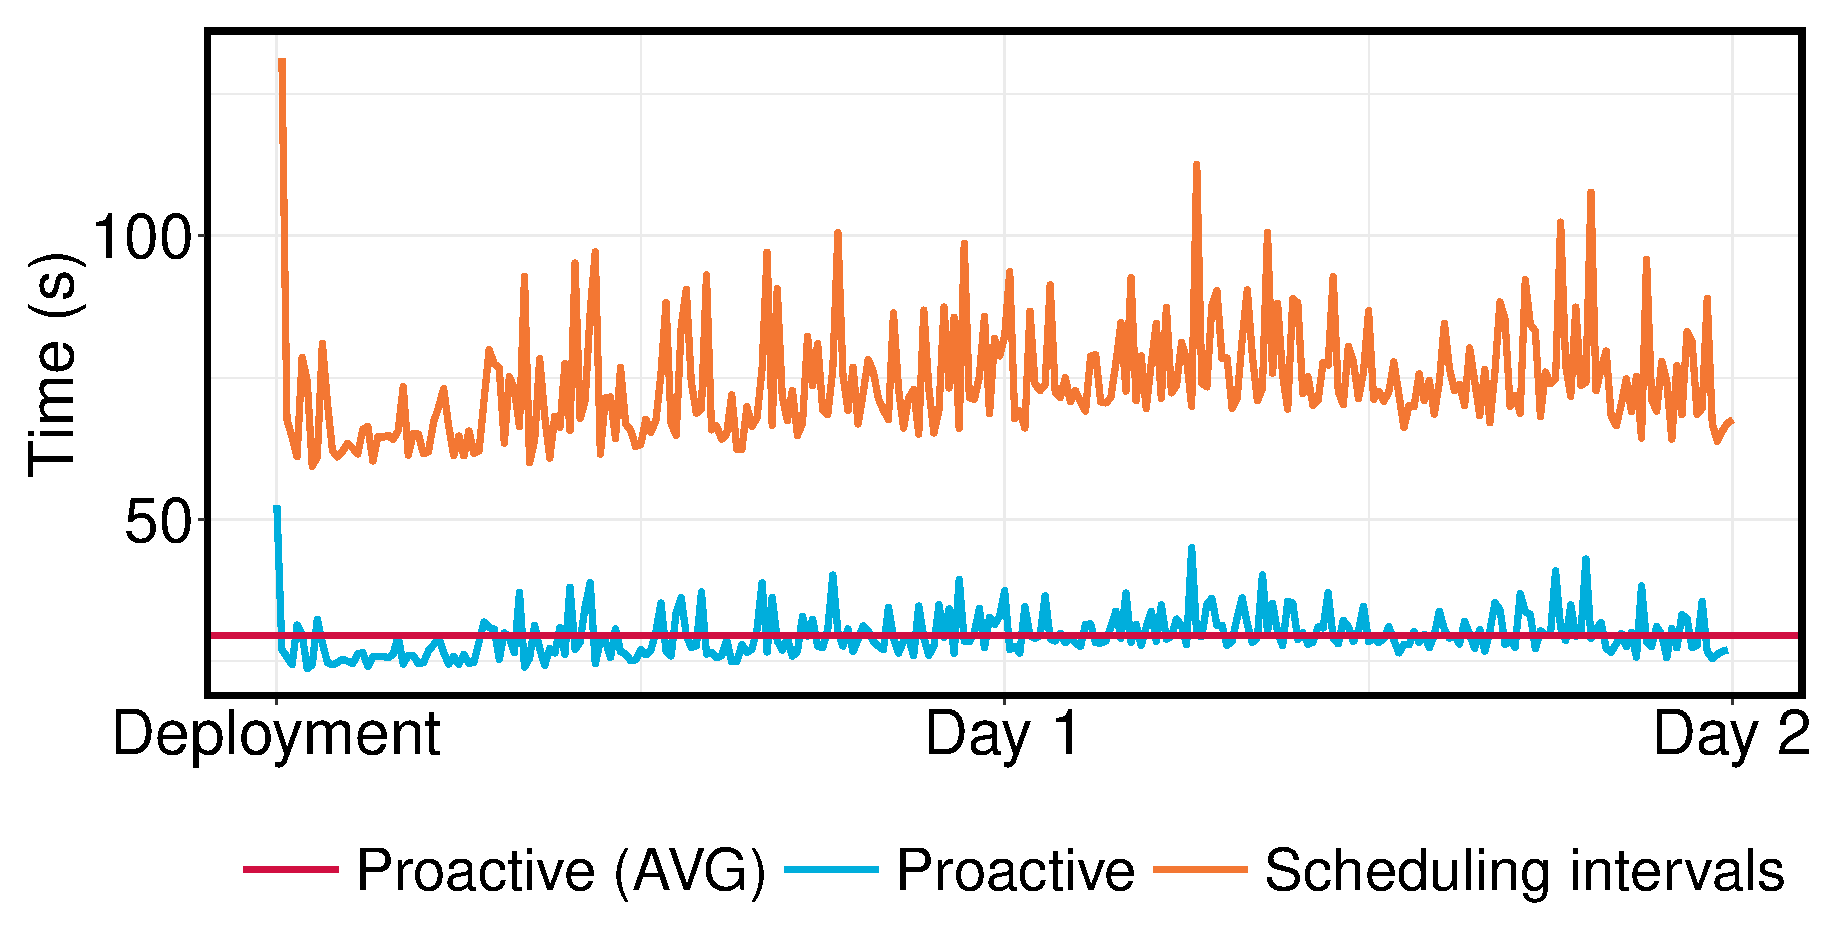
\includegraphics[width=\columnwidth]{../images/experiment-results/criteo-scheduling-experiment.eps}
%\caption{Analysis of scheduling policy}
%\label{fig:scheduling-policy-time}
%\vspace{2mm}
%\end{figure}
%
%Using the slack parameter, we can guide the scheduler to increase or decrease the scheduling intervals of the proactive training.
%The slack parameter allows for the deployment platform to accommodate surges in the incoming prediction requests and new training data.
%In scenarios where sudden surges are expected (e.g., online stores), we recommend a large slack parameter (recommended value is $10$). \todo[inline]{No exp. validate this}

\subsection{EX3: Optimizations Effects}
In this experiment, we analyze the effects of the optimizations, live statistics analysis and materialization of features, on the end-to-end deployment time.
Figure \ref{optimization-effect} shows the effect of optimizations on total training time.
By materializing the features, new instances of the proactive training have access directly to the preprocessed data.
As a result, proactive training directly computes the gradient and updates the deployed model.
For the URL pipeline, our optimizations have reduced the continuous training time by 50\%.
\hl{I will update Figure} \ref{optimization-effect} \hl{and show the time for every component of the pipeline and how the optimizations helped in reducing the time.}
\begin{figure}[h!]
\centering
\resizebox{\columnwidth}{!}{% Created by tikzDevice version 0.11 on 2018-04-23 15:52:24
% !TEX encoding = UTF-8 Unicode
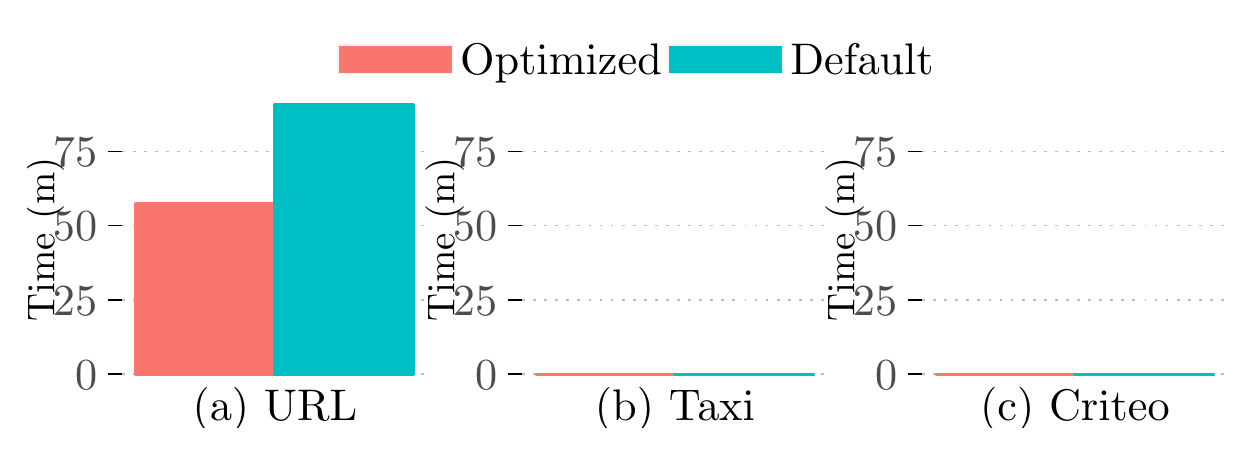
\begin{tikzpicture}[x=1pt,y=1pt]
\definecolor{fillColor}{RGB}{255,255,255}
\path[use as bounding box,fill=fillColor,fill opacity=0.00] (0,0) rectangle (433.62,144.54);
\begin{scope}
\path[clip] (  0.00,  0.00) rectangle (433.62,144.54);
\definecolor{fillColor}{RGB}{255,255,255}

\path[fill=fillColor] (101.43,121.66) rectangle (332.19,144.54);
\end{scope}
\begin{scope}
\path[clip] (  0.00,  0.00) rectangle (433.62,144.54);
\definecolor{drawColor}{RGB}{0,0,0}

\node[text=drawColor,anchor=base west,inner sep=0pt, outer sep=0pt, scale=  0.00] at (107.12,133.10) {Deployment};
\end{scope}
\begin{scope}
\path[clip] (  0.00,  0.00) rectangle (433.62,144.54);
\definecolor{drawColor}{RGB}{255,255,255}
\definecolor{fillColor}{gray}{0.95}

\path[draw=drawColor,line width= 0.6pt,line join=round,line cap=round,fill=fillColor] (111.46,127.35) rectangle (154.14,138.85);
\end{scope}
\begin{scope}
\path[clip] (  0.00,  0.00) rectangle (433.62,144.54);
\definecolor{drawColor}{RGB}{248,118,109}
\definecolor{fillColor}{RGB}{248,118,109}

\path[draw=drawColor,line width= 1.1pt,line cap=round,fill=fillColor] (112.88,128.78) rectangle (152.71,137.43);
\end{scope}
\begin{scope}
\path[clip] (  0.00,  0.00) rectangle (433.62,144.54);
\definecolor{drawColor}{RGB}{255,255,255}
\definecolor{fillColor}{gray}{0.95}

\path[draw=drawColor,line width= 0.6pt,line join=round,line cap=round,fill=fillColor] (230.77,127.35) rectangle (273.45,138.85);
\end{scope}
\begin{scope}
\path[clip] (  0.00,  0.00) rectangle (433.62,144.54);
\definecolor{drawColor}{RGB}{0,191,196}
\definecolor{fillColor}{RGB}{0,191,196}

\path[draw=drawColor,line width= 1.1pt,line cap=round,fill=fillColor] (232.19,128.78) rectangle (272.02,137.43);
\end{scope}
\begin{scope}
\path[clip] (  0.00,  0.00) rectangle (433.62,144.54);
\definecolor{drawColor}{RGB}{0,0,0}

\node[text=drawColor,anchor=base west,inner sep=0pt, outer sep=0pt, scale=  1.60] at (156.30,127.59) {Optimized};
\end{scope}
\begin{scope}
\path[clip] (  0.00,  0.00) rectangle (433.62,144.54);
\definecolor{drawColor}{RGB}{0,0,0}

\node[text=drawColor,anchor=base west,inner sep=0pt, outer sep=0pt, scale=  1.60] at (275.61,127.59) {Default};
\end{scope}
\begin{scope}
\path[clip] (  0.00,  0.00) rectangle (144.54,121.66);
\definecolor{drawColor}{RGB}{255,255,255}
\definecolor{fillColor}{RGB}{255,255,255}

\path[draw=drawColor,line width= 0.6pt,line join=round,line cap=round,fill=fillColor] (  0.00, -0.00) rectangle (144.54,121.66);
\end{scope}
\begin{scope}
\path[clip] ( 34.13, 14.51) rectangle (144.54,121.66);
\definecolor{fillColor}{RGB}{255,255,255}

\path[fill=fillColor] ( 34.13, 14.51) rectangle (144.54,121.66);
\definecolor{drawColor}{RGB}{255,255,255}

\path[draw=drawColor,line width= 0.3pt,line join=round] ( 34.13, 32.79) --
	(144.54, 32.79);

\path[draw=drawColor,line width= 0.3pt,line join=round] ( 34.13, 59.60) --
	(144.54, 59.60);

\path[draw=drawColor,line width= 0.3pt,line join=round] ( 34.13, 86.41) --
	(144.54, 86.41);

\path[draw=drawColor,line width= 0.3pt,line join=round] ( 34.13,113.22) --
	(144.54,113.22);
\definecolor{drawColor}{RGB}{190,190,190}

\path[draw=drawColor,line width= 0.6pt,dash pattern=on 1pt off 3pt ,line join=round] ( 34.13, 19.38) --
	(144.54, 19.38);

\path[draw=drawColor,line width= 0.6pt,dash pattern=on 1pt off 3pt ,line join=round] ( 34.13, 46.19) --
	(144.54, 46.19);

\path[draw=drawColor,line width= 0.6pt,dash pattern=on 1pt off 3pt ,line join=round] ( 34.13, 73.00) --
	(144.54, 73.00);

\path[draw=drawColor,line width= 0.6pt,dash pattern=on 1pt off 3pt ,line join=round] ( 34.13, 99.81) --
	(144.54, 99.81);
\definecolor{drawColor}{RGB}{255,255,255}

\path[draw=drawColor,line width= 0.6pt,line join=round] ( 64.24, 14.51) --
	( 64.24,121.66);

\path[draw=drawColor,line width= 0.6pt,line join=round] (114.43, 14.51) --
	(114.43,121.66);
\definecolor{drawColor}{RGB}{248,118,109}
\definecolor{fillColor}{RGB}{248,118,109}

\path[draw=drawColor,line width= 1.1pt,line join=round,fill=fillColor] ( 39.15, 19.38) rectangle ( 89.34, 80.88);
\definecolor{drawColor}{RGB}{0,191,196}
\definecolor{fillColor}{RGB}{0,191,196}

\path[draw=drawColor,line width= 1.1pt,line join=round,fill=fillColor] ( 89.34, 19.38) rectangle (139.52,116.79);
\end{scope}
\begin{scope}
\path[clip] (  0.00,  0.00) rectangle (433.62,144.54);
\definecolor{drawColor}{gray}{0.30}

\node[text=drawColor,anchor=base east,inner sep=0pt, outer sep=0pt, scale=  1.60] at ( 25.13, 13.87) {0};

\node[text=drawColor,anchor=base east,inner sep=0pt, outer sep=0pt, scale=  1.60] at ( 25.13, 40.68) {25};

\node[text=drawColor,anchor=base east,inner sep=0pt, outer sep=0pt, scale=  1.60] at ( 25.13, 67.49) {50};

\node[text=drawColor,anchor=base east,inner sep=0pt, outer sep=0pt, scale=  1.60] at ( 25.13, 94.30) {75};
\end{scope}
\begin{scope}
\path[clip] (  0.00,  0.00) rectangle (433.62,144.54);
\definecolor{drawColor}{RGB}{0,0,0}

\path[draw=drawColor,line width= 0.6pt,line join=round] ( 29.13, 19.38) --
	( 34.13, 19.38);

\path[draw=drawColor,line width= 0.6pt,line join=round] ( 29.13, 46.19) --
	( 34.13, 46.19);

\path[draw=drawColor,line width= 0.6pt,line join=round] ( 29.13, 73.00) --
	( 34.13, 73.00);

\path[draw=drawColor,line width= 0.6pt,line join=round] ( 29.13, 99.81) --
	( 34.13, 99.81);
\end{scope}
\begin{scope}
\path[clip] (  0.00,  0.00) rectangle (433.62,144.54);
\definecolor{drawColor}{RGB}{0,0,0}

\node[text=drawColor,anchor=base,inner sep=0pt, outer sep=0pt, scale=  1.60] at ( 89.34,  2.49) {(a) URL};
\end{scope}
\begin{scope}
\path[clip] (  0.00,  0.00) rectangle (433.62,144.54);
\definecolor{drawColor}{RGB}{0,0,0}

\node[text=drawColor,rotate= 90.00,anchor=base,inner sep=0pt, outer sep=0pt, scale=  1.40] at (  9.64, 68.09) {Time (m)};
\end{scope}
\begin{scope}
\path[clip] (144.54,  0.00) rectangle (289.08,121.66);
\definecolor{drawColor}{RGB}{255,255,255}
\definecolor{fillColor}{RGB}{255,255,255}

\path[draw=drawColor,line width= 0.6pt,line join=round,line cap=round,fill=fillColor] (144.54, -0.00) rectangle (289.08,121.66);
\end{scope}
\begin{scope}
\path[clip] (178.67, 14.51) rectangle (289.08,121.66);
\definecolor{fillColor}{RGB}{255,255,255}

\path[fill=fillColor] (178.67, 14.51) rectangle (289.08,121.66);
\definecolor{drawColor}{RGB}{255,255,255}

\path[draw=drawColor,line width= 0.3pt,line join=round] (178.67, 32.79) --
	(289.08, 32.79);

\path[draw=drawColor,line width= 0.3pt,line join=round] (178.67, 59.60) --
	(289.08, 59.60);

\path[draw=drawColor,line width= 0.3pt,line join=round] (178.67, 86.41) --
	(289.08, 86.41);

\path[draw=drawColor,line width= 0.3pt,line join=round] (178.67,113.22) --
	(289.08,113.22);
\definecolor{drawColor}{RGB}{190,190,190}

\path[draw=drawColor,line width= 0.6pt,dash pattern=on 1pt off 3pt ,line join=round] (178.67, 19.38) --
	(289.08, 19.38);

\path[draw=drawColor,line width= 0.6pt,dash pattern=on 1pt off 3pt ,line join=round] (178.67, 46.19) --
	(289.08, 46.19);

\path[draw=drawColor,line width= 0.6pt,dash pattern=on 1pt off 3pt ,line join=round] (178.67, 73.00) --
	(289.08, 73.00);

\path[draw=drawColor,line width= 0.6pt,dash pattern=on 1pt off 3pt ,line join=round] (178.67, 99.81) --
	(289.08, 99.81);
\definecolor{drawColor}{RGB}{255,255,255}

\path[draw=drawColor,line width= 0.6pt,line join=round] (208.78, 14.51) --
	(208.78,121.66);

\path[draw=drawColor,line width= 0.6pt,line join=round] (258.97, 14.51) --
	(258.97,121.66);
\definecolor{drawColor}{RGB}{248,118,109}
\definecolor{fillColor}{RGB}{248,118,109}

\path[draw=drawColor,line width= 1.1pt,line join=round,fill=fillColor] (183.69, 19.38) rectangle (233.88, 19.38);
\definecolor{drawColor}{RGB}{0,191,196}
\definecolor{fillColor}{RGB}{0,191,196}

\path[draw=drawColor,line width= 1.1pt,line join=round,fill=fillColor] (233.88, 19.38) rectangle (284.06, 19.38);
\end{scope}
\begin{scope}
\path[clip] (  0.00,  0.00) rectangle (433.62,144.54);
\definecolor{drawColor}{gray}{0.30}

\node[text=drawColor,anchor=base east,inner sep=0pt, outer sep=0pt, scale=  1.60] at (169.67, 13.87) {0};

\node[text=drawColor,anchor=base east,inner sep=0pt, outer sep=0pt, scale=  1.60] at (169.67, 40.68) {25};

\node[text=drawColor,anchor=base east,inner sep=0pt, outer sep=0pt, scale=  1.60] at (169.67, 67.49) {50};

\node[text=drawColor,anchor=base east,inner sep=0pt, outer sep=0pt, scale=  1.60] at (169.67, 94.30) {75};
\end{scope}
\begin{scope}
\path[clip] (  0.00,  0.00) rectangle (433.62,144.54);
\definecolor{drawColor}{RGB}{0,0,0}

\path[draw=drawColor,line width= 0.6pt,line join=round] (173.67, 19.38) --
	(178.67, 19.38);

\path[draw=drawColor,line width= 0.6pt,line join=round] (173.67, 46.19) --
	(178.67, 46.19);

\path[draw=drawColor,line width= 0.6pt,line join=round] (173.67, 73.00) --
	(178.67, 73.00);

\path[draw=drawColor,line width= 0.6pt,line join=round] (173.67, 99.81) --
	(178.67, 99.81);
\end{scope}
\begin{scope}
\path[clip] (  0.00,  0.00) rectangle (433.62,144.54);
\definecolor{drawColor}{RGB}{0,0,0}

\node[text=drawColor,anchor=base,inner sep=0pt, outer sep=0pt, scale=  1.60] at (233.88,  2.49) {(b) Taxi};
\end{scope}
\begin{scope}
\path[clip] (  0.00,  0.00) rectangle (433.62,144.54);
\definecolor{drawColor}{RGB}{0,0,0}

\node[text=drawColor,rotate= 90.00,anchor=base,inner sep=0pt, outer sep=0pt, scale=  1.40] at (154.18, 68.09) {Time (m)};
\end{scope}
\begin{scope}
\path[clip] (289.08,  0.00) rectangle (433.62,121.66);
\definecolor{drawColor}{RGB}{255,255,255}
\definecolor{fillColor}{RGB}{255,255,255}

\path[draw=drawColor,line width= 0.6pt,line join=round,line cap=round,fill=fillColor] (289.08, -0.00) rectangle (433.62,121.66);
\end{scope}
\begin{scope}
\path[clip] (323.21, 14.51) rectangle (433.62,121.66);
\definecolor{fillColor}{RGB}{255,255,255}

\path[fill=fillColor] (323.21, 14.51) rectangle (433.62,121.66);
\definecolor{drawColor}{RGB}{255,255,255}

\path[draw=drawColor,line width= 0.3pt,line join=round] (323.21, 32.79) --
	(433.62, 32.79);

\path[draw=drawColor,line width= 0.3pt,line join=round] (323.21, 59.60) --
	(433.62, 59.60);

\path[draw=drawColor,line width= 0.3pt,line join=round] (323.21, 86.41) --
	(433.62, 86.41);

\path[draw=drawColor,line width= 0.3pt,line join=round] (323.21,113.22) --
	(433.62,113.22);
\definecolor{drawColor}{RGB}{190,190,190}

\path[draw=drawColor,line width= 0.6pt,dash pattern=on 1pt off 3pt ,line join=round] (323.21, 19.38) --
	(433.62, 19.38);

\path[draw=drawColor,line width= 0.6pt,dash pattern=on 1pt off 3pt ,line join=round] (323.21, 46.19) --
	(433.62, 46.19);

\path[draw=drawColor,line width= 0.6pt,dash pattern=on 1pt off 3pt ,line join=round] (323.21, 73.00) --
	(433.62, 73.00);

\path[draw=drawColor,line width= 0.6pt,dash pattern=on 1pt off 3pt ,line join=round] (323.21, 99.81) --
	(433.62, 99.81);
\definecolor{drawColor}{RGB}{255,255,255}

\path[draw=drawColor,line width= 0.6pt,line join=round] (353.32, 14.51) --
	(353.32,121.66);

\path[draw=drawColor,line width= 0.6pt,line join=round] (403.51, 14.51) --
	(403.51,121.66);
\definecolor{drawColor}{RGB}{248,118,109}
\definecolor{fillColor}{RGB}{248,118,109}

\path[draw=drawColor,line width= 1.1pt,line join=round,fill=fillColor] (328.23, 19.38) rectangle (378.42, 19.38);
\definecolor{drawColor}{RGB}{0,191,196}
\definecolor{fillColor}{RGB}{0,191,196}

\path[draw=drawColor,line width= 1.1pt,line join=round,fill=fillColor] (378.42, 19.38) rectangle (428.60, 19.38);
\end{scope}
\begin{scope}
\path[clip] (  0.00,  0.00) rectangle (433.62,144.54);
\definecolor{drawColor}{gray}{0.30}

\node[text=drawColor,anchor=base east,inner sep=0pt, outer sep=0pt, scale=  1.60] at (314.21, 13.87) {0};

\node[text=drawColor,anchor=base east,inner sep=0pt, outer sep=0pt, scale=  1.60] at (314.21, 40.68) {25};

\node[text=drawColor,anchor=base east,inner sep=0pt, outer sep=0pt, scale=  1.60] at (314.21, 67.49) {50};

\node[text=drawColor,anchor=base east,inner sep=0pt, outer sep=0pt, scale=  1.60] at (314.21, 94.30) {75};
\end{scope}
\begin{scope}
\path[clip] (  0.00,  0.00) rectangle (433.62,144.54);
\definecolor{drawColor}{RGB}{0,0,0}

\path[draw=drawColor,line width= 0.6pt,line join=round] (318.21, 19.38) --
	(323.21, 19.38);

\path[draw=drawColor,line width= 0.6pt,line join=round] (318.21, 46.19) --
	(323.21, 46.19);

\path[draw=drawColor,line width= 0.6pt,line join=round] (318.21, 73.00) --
	(323.21, 73.00);

\path[draw=drawColor,line width= 0.6pt,line join=round] (318.21, 99.81) --
	(323.21, 99.81);
\end{scope}
\begin{scope}
\path[clip] (  0.00,  0.00) rectangle (433.62,144.54);
\definecolor{drawColor}{RGB}{0,0,0}

\node[text=drawColor,anchor=base,inner sep=0pt, outer sep=0pt, scale=  1.60] at (378.42,  2.49) {(c) Criteo};
\end{scope}
\begin{scope}
\path[clip] (  0.00,  0.00) rectangle (433.62,144.54);
\definecolor{drawColor}{RGB}{0,0,0}

\node[text=drawColor,rotate= 90.00,anchor=base,inner sep=0pt, outer sep=0pt, scale=  1.40] at (298.72, 68.09) {Time (m)};
\end{scope}
\end{tikzpicture}
}
\caption{Effect of the optimizations on total training time in continuous deployment approach}
\label{optimization-effect}
\end{figure}

\subsection{Discussion} \label{subsec:discussion}
\todo[inline]{Maybe I can also add the result of the scheduling experiment}
\todo[inline]{Explain it is always possible to train the model further and may achieve better result in periodical deployment by given the same amount of time in tuning and designing a pipeline, continuous performs better.}
\textbf{Side effect of periodical deployment.}
In our experiments, incoming predictions where paused until the end of a periodical training.
However, in real-world scenarios, prediction queries arrive constantly arrive at the system.
Therefore, prediction queries are answered by the model before the periodical training was initiated. 
Moreover, during the periodical training, the model cannot be updated using online learning algorithm as well.
As a result, the performance of the model while a new model is being trained does not improve.
The average training time for the proactive training is very small (200 ms for the URL pipeline \hl{nyc and criteo}).
Therefore, predictions queries are always answered by an up-to-date model and online learning is not paused in the continuous deployment.


